\documentclass[a4paper,11pt,openany]{book}

% Pacchetti essenziali
\usepackage[utf8]{inputenc}
\usepackage[T1]{fontenc}
\usepackage[italian]{babel}
\usepackage{geometry}
\usepackage{graphicx}
\usepackage{float}
\usepackage{caption}
\usepackage{subcaption}
\usepackage{amsmath}
\usepackage{amsfonts}
\usepackage{amssymb}
\usepackage{xcolor}
\usepackage{listings}
\usepackage{fancyhdr}
\usepackage{titlesec}
\usepackage{tocloft}
\usepackage{hyperref}
\usepackage{booktabs}
\usepackage{longtable}
\usepackage{array}
\usepackage{multirow}
\usepackage{tikz}
\usepackage{pgfplots}
\usepackage{musicography}

% Configurazione geometria pagina
\geometry{
    left=2.5cm,
    right=2cm,
    top=2.5cm,
    bottom=2.5cm,
    headheight=14pt
}

% Configurazione colori
\definecolor{granixblue}{RGB}{0,10,160}
\definecolor{granixcyan}{RGB}{0,255,255}
\definecolor{granixwhite}{RGB}{255,255,255}

% Configurazione hyperref
\hypersetup{
    colorlinks=true,
    linkcolor=granixblue,
    urlcolor=granixblue,
    citecolor=granixblue,
    pdfauthor={Francesco Dicorato},
    pdftitle={GRANIX - Granulatore Ambisonico - Manuale Utente},
    pdfsubject={Audio Granular Synthesis and Ambisonics},
    pdfkeywords={Granular Synthesis, Ambisonics, Csound, Audio Processing}
}

% Configurazione header e footer
\pagestyle{fancy}
\fancyhf{}
\fancyhead[LE]{\leftmark}
\fancyhead[RO]{\rightmark}
\fancyfoot[C]{\thepage}
\renewcommand{\headrulewidth}{0.4pt}

% Configurazione capitoli e sezioni
\titleformat{\chapter}[display]
    {\normalfont\huge\bfseries\color{granixblue}}
    {\chaptertitlename\ \thechapter}{20pt}{\Huge}
\titleformat{\section}
    {\normalfont\Large\bfseries\color{granixblue}}
    {\thesection}{1em}{}
\titleformat{\subsection}
    {\normalfont\large\bfseries\color{granixblue}}
    {\thesubsection}{1em}{}

% Configurazione listings per codice
\lstset{
    basicstyle=\ttfamily\small,
    backgroundcolor=\color{gray!10},
    frame=single,
    language=C,
    keywordstyle=\color{granixblue}\bfseries,
    commentstyle=\color{gray}\itshape,
    numbers=left,
    numberstyle=\tiny\color{gray},
    breaklines=true,
    tabsize=2
}

% Configurazione didascalie
\captionsetup{
    font=small,
    labelfont=bf,
    textfont=it,
    format=hang,
    margin=10pt
}

% Comandi personalizzati
\newcommand{\granix}{\textbf{\textcolor{granixblue}{GRANIX}}}
\newcommand{\ambisonics}{\textit{Ambisonics}}
\newcommand{\foa}{\textsc{foa}}
\newcommand{\ambix}{\textsc{AmbiX}}
\newcommand{\csound}{\texttt{Csound}}
\newcommand{\cabbage}{\texttt{Cabbage}}

% Ambiente per parametri tecnici
\newenvironment{parambox}[1]{
    \begin{center}
    \begin{tabular}{|p{0.9\textwidth}|}
    \hline
    \textbf{#1} \\
    \hline
}{
    \hline
    \end{tabular}
    \end{center}
}

% Ambiente per esempi pratici
\newenvironment{esempio}[1]{
    \begin{figure}[H]
    \centering
    \fcolorbox{granixblue}{gray!5}{
        \begin{minipage}{0.9\textwidth}
        \textbf{\textcolor{granixblue}{Esempio: #1}}
        \vspace{0.5em}
        
}{
        \end{minipage}
    }
    \end{figure}
}

\begin{document}

% Pagina del titolo
\begin{titlepage}
    \centering
    \vspace*{2cm}
    
    % Logo placeholder
    
\includegraphics[width=0.8\textwidth]{img/GRANIX_logo.png} % Aggiungi il tuo logo
    
    \vspace{1.5cm}
    
    {\Huge\bfseries\color{granixblue} GRANIX}
    
    \vspace{0.5cm}
    
    {\Large\textit{Granulatore Ambisonico}}
    
    \vspace{1cm}
    
    {\large Manuale Utente e Guida Tecnica}
    
    \vspace{2cm}
    
    \begin{figure}[H]
        \centering
        % Placeholder per screenshot principale dell'interfaccia
        \fbox{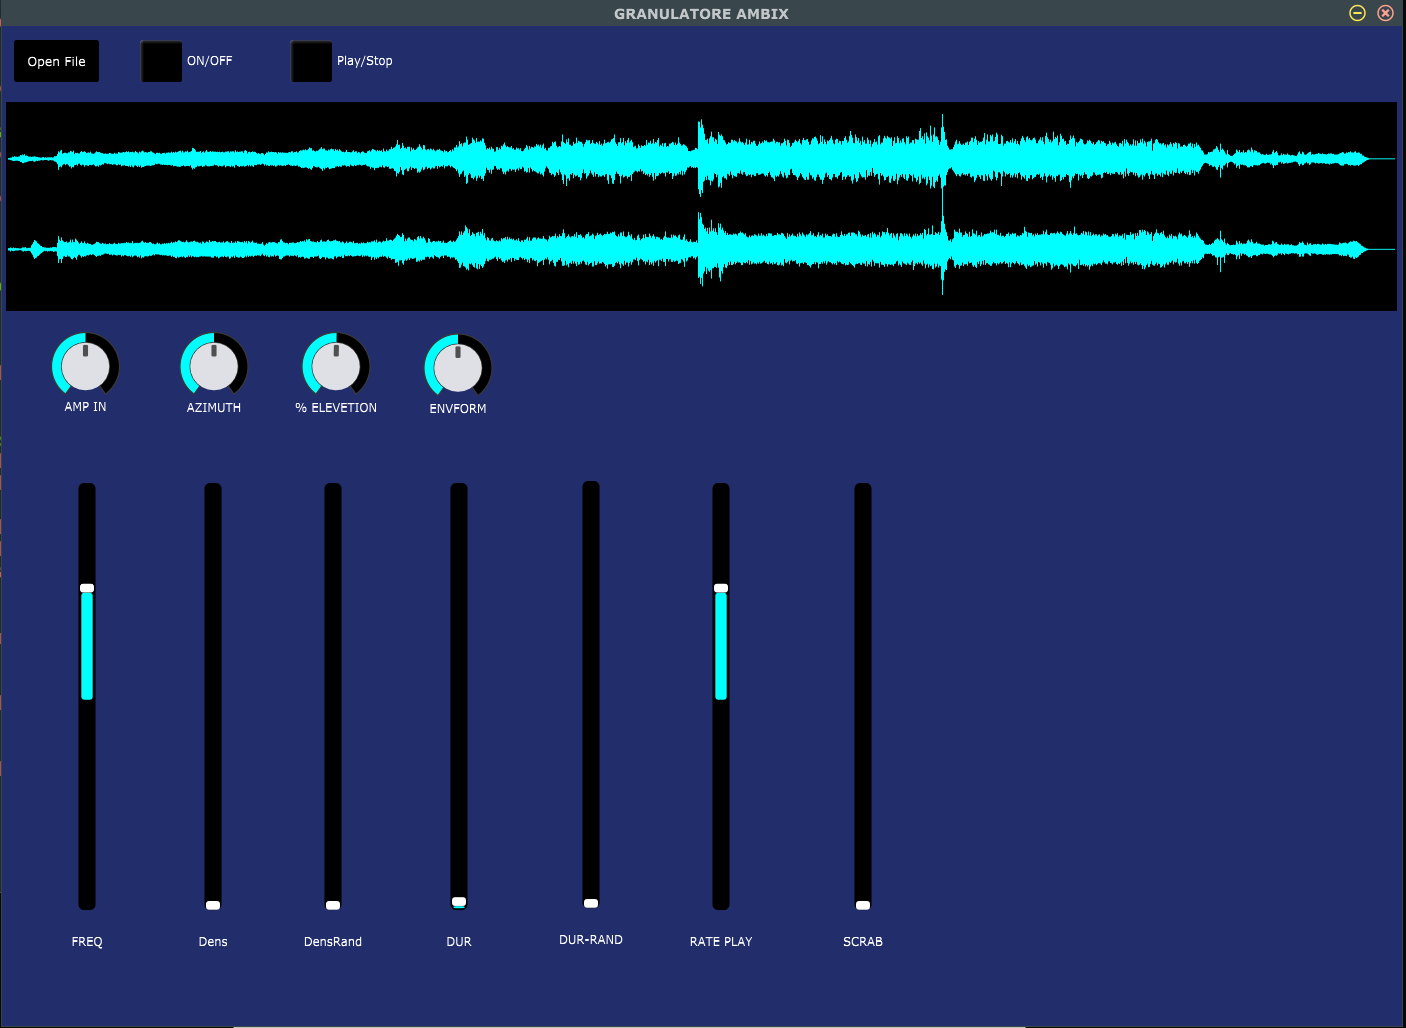
\includegraphics[width=1.0\textwidth]{img/GUI/GUI NUOVA Buff pieno.PNG}}
        \caption*{Interfaccia principale di \granix}
    \end{figure}
    
    \vfill
    
    {\large Francesco Dicorato}
    
    \vspace{0.5cm}
    
    {\large \today}
    
\end{titlepage}

% Copyright e informazioni
\newpage
\thispagestyle{empty}
\vspace*{\fill}
\begin{center}
\textbf{\granix\ - Granulatore Ambisonico}\\
Manuale Utente e Guida Tecnica\\
\vspace{1cm}
Copyright \textcopyright\ 2025 Francesco Dicorato\\
\vspace{0.5cm}
Questo documento è distribuito sotto licenza Creative Commons\\
Attribution-ShareAlike 4.0 International (CC BY-SA 4.0)\\
\vspace{1cm}
Sviluppato con \csound\ e \cabbage\\
Per informazioni e aggiornamenti: \url{https://github.com/username/granix}
\end{center}
\vspace*{\fill}

% Indice
\tableofcontents
\newpage

% Lista delle figure
\listoffigures
\newpage

% Lista delle tabelle
\listoftables
\newpage

% Prefazione
\chapter*{Prefazione}
\addcontentsline{toc}{chapter}{Prefazione}

\granix\ è un plug-in VST3(Virtual Studio Technology) programmato in linguaggio Csound e sviluppato all'interno del framework Cabbage. L'idea creativa che lo distingue, rendendolo unico rispetto ad altri granulatori risiede nella gestione ragionata e controllata dell'output spaziale dei grani, attraverso il formato ambisonics  di primo ordine standard AmbiX. Questo strumento trascende il concetto tradizionale di granulazione come semplice effetto audio, trasformandosi in un vero e proprio ambiente compositivo dove lo spazio diventa elemento costitutivo dell'esperienza sonora.

Il presente manuale si propone di guidare l'utente attraverso tutti gli aspetti del software, dalla comprensione teorica dei principi di base fino alle tecniche avanzate di performance e composizione. Ogni sezione è corredata da esempi pratici, screenshot dettagliati e riferimenti tecnici per fornire una comprensione completa dello strumento.


\vspace{1cm}

\textit{Francesco Dicorato}\\
\textit{Bari, 2025}

\chapter{Introduzione alla Sintesi Granulare}

\section{Fondamenti Teorici}

La \textbf{sintesi granulare} costituisce una delle tecniche più innovative e versatili nell'ambito dell'elaborazione audio digitale. Il termine deriva dal latino \textit{granulum}, diminutivo di \textit{granum} (chicco, grano), evidenziando la natura particellare e frammentaria di questa metodologia di sintesi.

\begin{figure}[H]
    \centering
    % Placeholder per diagramma concettuale della granulazione
    \fbox{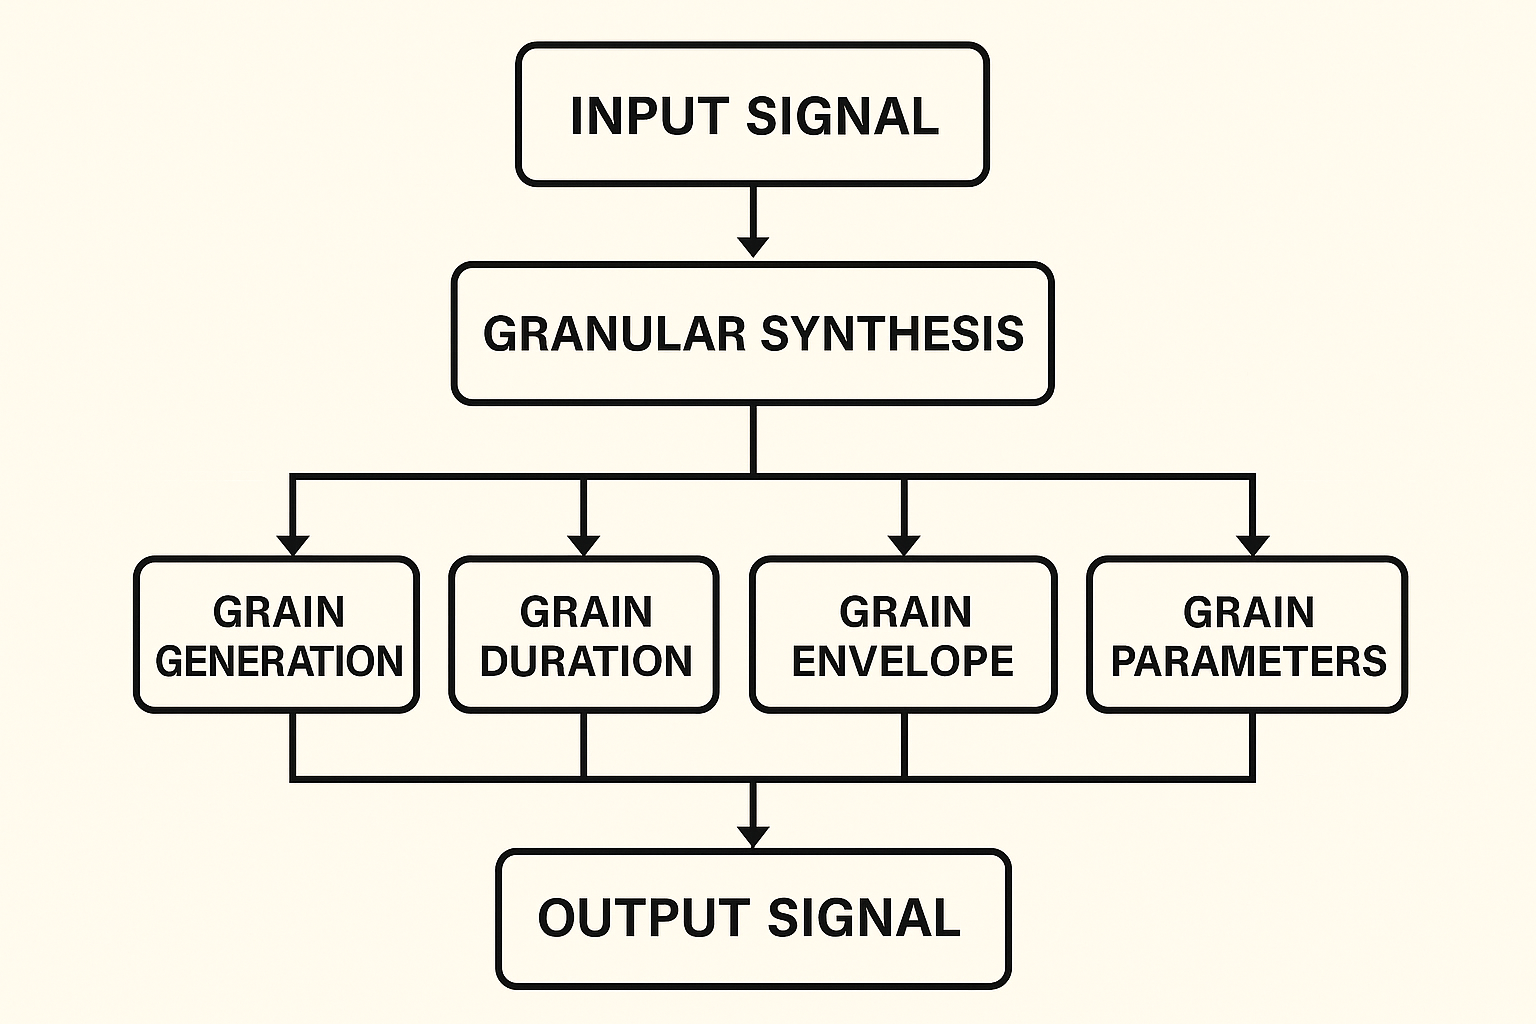
\includegraphics[width=0.8\textwidth]{img/schema_concettuale_grani.png}}
    \caption{Schema concettuale della sintesi granulare}
    \label{fig:granular_concept}
\end{figure}

La tecnica si basa sulla scomposizione del materiale sonoro in piccoli frammenti temporali chiamati \textbf{grani} (grains), tipicamente compresi tra 1 e 100 millisecondi. Ogni grano viene processato individualmente secondo parametri specifici e successivamente ricombinato con altri grani per generare nuove texture sonore.

\subsection{Storia e Sviluppo}

La sintesi granulare ha le sue radici teoriche nei lavori di Dennis Gabor negli anni '40, che propose la decomposizione del suono in "quanti acustici". Il concetto fu successivamente sviluppato da Iannis Xenakis negli anni '70 e implementato digitalmente da Curtis Roads e Barry Truax negli anni '80.

\subsection{Principi Operativi}

\subsubsection{Anatomia del Grano}

Ogni grano sonoro è caratterizzato da quattro parametri fondamentali:

\begin{enumerate}
    \item \textbf{Durata}: L'estensione temporale del grano, solitamente tra 1-100ms
    \item \textbf{Inviluppo}: La forma dell'ampiezza nel tempo (attacco, sustain, rilascio)
    \item \textbf{Posizione}: Il punto di origine nel materiale sorgente
    \item \textbf{Trasposizione}: La velocità di riproduzione (controllo del pitch)
\end{enumerate}

\begin{figure}[H]
    \centering
    % Placeholder per diagramma dell'anatomia del grano
    \fbox{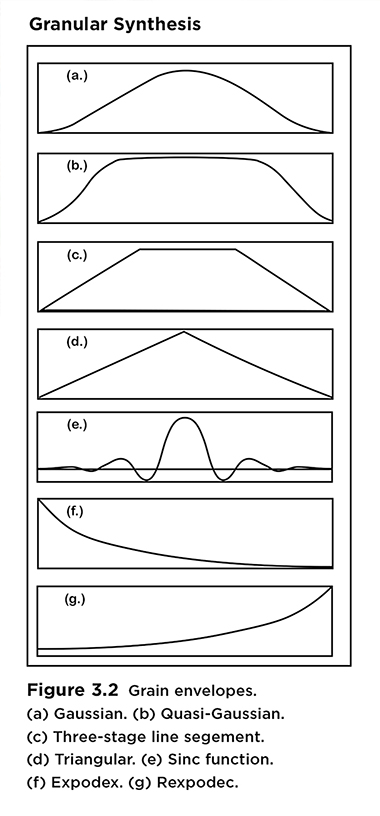
\includegraphics[width=0.6\textwidth]{img/GrainEnvelopes.jpg}}
    \caption{Struttura di un singolo grano con vari inviluppi, ripresi da "Microsound" di C.Road}
    \label{fig:grain_anatomy}
\end{figure}

\subsubsection{Densità Granulare}

La \textbf{densità} rappresenta il numero di grani generati per unità di tempo, tipicamente espressa in grani per secondo (grains/sec). Questo parametro determina la natura percettiva del risultato:

\begin{itemize}
    \item \textbf{Bassa densità} (1-10 grani/sec): Effetti ritmici discreti
    \item \textbf{Media densità} (20-50 grani/sec): Texture granulari riconoscibili
    \item \textbf{Alta densità} (100+ grani/sec): Flussi sonori continui
\end{itemize}

\section{Applicazioni Creative}

\subsection{Time-stretching e Pitch-shifting}

La granulazione permette di manipolare indipendentemente durata e altezza del materiale sonoro:

%\begin{exemplo}{Time-stretching}
\textbf{Parametri:}
\begin{itemize}
    \item Densità: 100 grani/sec
    \item Durata grano: 50ms
    \item Velocità lettura: 0.5x (metà velocità)
    \item Trasposizione: 1.0 (pitch invariato)
\end{itemize}
\textbf{Risultato:} Audio esteso al doppio della durata originale senza alterazione del pitch.
%\end{exemplo}

\subsection{Creazione di Texture}

La randomizzazione dei parametri granulari genera complesse texture sonore impossibili da ottenere con tecniche tradizionali.

\begin{figure}[H]
    \centering
    % Placeholder per spettrogramma di texture granulare
    \fbox{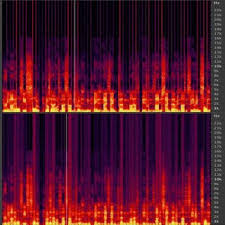
\includegraphics[width=0.8\textwidth]{img/Spettro.jpg}}
    \caption{Analisi spettrale di una texture granulare complessa}
    \label{fig:granular_texture}
\end{figure}

\chapter{Ambisonics e Spazializzazione Audio}

\section{Introduzione agli \ambisonics}

Il termine \ambisonics\ deriva dalla combinazione del prefisso greco \textit{ambi-} (intorno, circostante) e del latino \textit{sonus} (suono), indicando letteralmente "suono che circonda". Questo sistema di codifica audio tridimensionale, sviluppato da Michael Gerzon negli anni '70, rappresenta una delle metodologie più avanzate per la cattura, elaborazione e riproduzione di campi sonori spaziali.

\begin{figure}[H]
    \centering
    % Placeholder per diagramma sferico ambisonics
    \fbox{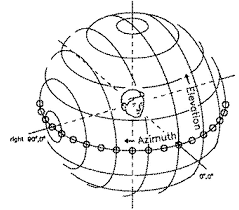
\includegraphics[width=0.6\textwidth]{img/campo_sonoro.png}}
    \caption{Rappresentazione sferica del campo sonoro \ambisonics}
    \label{fig:ambisonic_sphere}
\end{figure}

\subsection{Principi di Codifica Sferica}

Gli \ambisonics\ si basano sull'uso di \textbf{armoniche sferiche} per descrivere matematicamente la distribuzione direzionale dell'energia sonora su una superficie sferica. Questa rappresentazione permette una riproduzione accurata indipendentemente dalla configurazione degli altoparlanti utilizzati.

\section{Format \ambix\ di Primo Ordine}

\granix\ utilizza il formato \ambix\ di primo ordine (\foa), che impiega quattro canali per codificare il campo sonoro tridimensionale:

\begin{table}[H]
    \centering
    \caption{Canali \ambix\ di primo ordine}
    \label{tab:ambix_channels}
    \begin{tabular}{@{}clp{6cm}@{}}
        \toprule
        \textbf{Canale} & \textbf{Nome} & \textbf{Funzione} \\
        \midrule
        0 & W*sqrt(2) & Componente omnidirezionale (pressione sonora) \\
        1 & Y & Gradiente sinistra-destra (figura a otto orizzontale) \\
        2 & Z & Gradiente alto-basso (figura a otto verticale) \\
        3 & X & Gradiente avanti-dietro (figura a otto sagittale) \\
        \bottomrule
    \end{tabular}
\end{table}

\subsection{Coordinate Sferiche}

Il posizionamento spaziale utilizza un sistema di coordinate sferiche standard:

\begin{itemize}
    \item \textbf{Azimuth} ($\theta$): Angolo orizzontale, $-180° \leq \theta \leq +180°$
    \item \textbf{Elevation} ($\phi$): Angolo verticale, $-90° \leq \phi \leq +90°$
\end{itemize}

\begin{figure}[H]
    \centering
    % Placeholder per diagramma coordinate sferiche
    \fbox{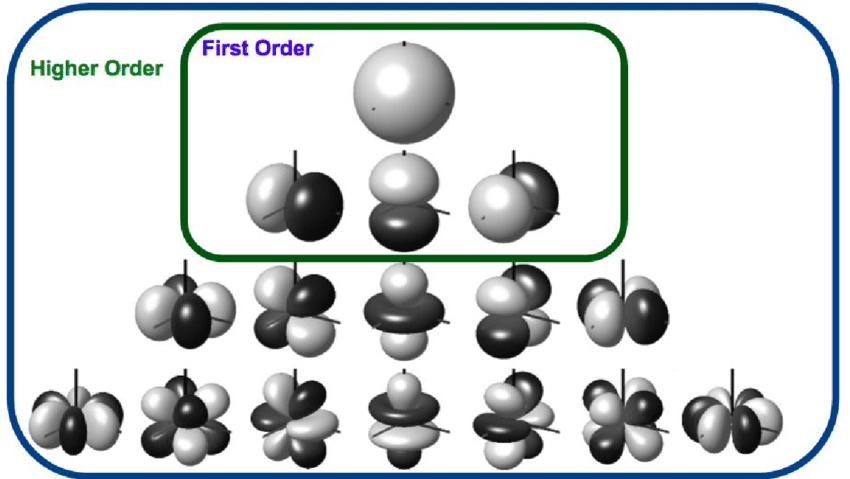
\includegraphics[width=0.7\textwidth]{img/sual-representation-of-ambisonics.png}}
    \caption{Sistema di coordinate sferiche per il posizionamento audio}
    \label{fig:spherical_coords}
\end{figure}

\subsection{Equazioni di Encoding}

La conversione da segnale mono-posizionato ai quattro canali \ambix\ segue le equazioni:

\begin{align}
W*sqrt(2) &= S \\
Y &= S \cdot \sin(\theta) \cdot \cos(\phi) \\
Z &= S \cdot \sin(\phi) \\
X &= S \cdot \cos(\theta) \cdot \cos(\phi)
\end{align}

dove $S$ rappresenta il segnale sorgente.

\section{Limitazioni e Artefatti del \foa}

\subsection{Effetto "Ciambella"}

Il formato di primo ordine presenta intrinsecamente una limitazione nota come \textit{effetto ciambella} o risoluzione direzionale limitata. Questo fenomeno si manifesta come zone di energia debole distribuite lungo archi curvi nello spazio sferico.

\begin{figure}[H]
    \centering
    % Placeholder per visualizzazione effetto ciambella
    \fbox{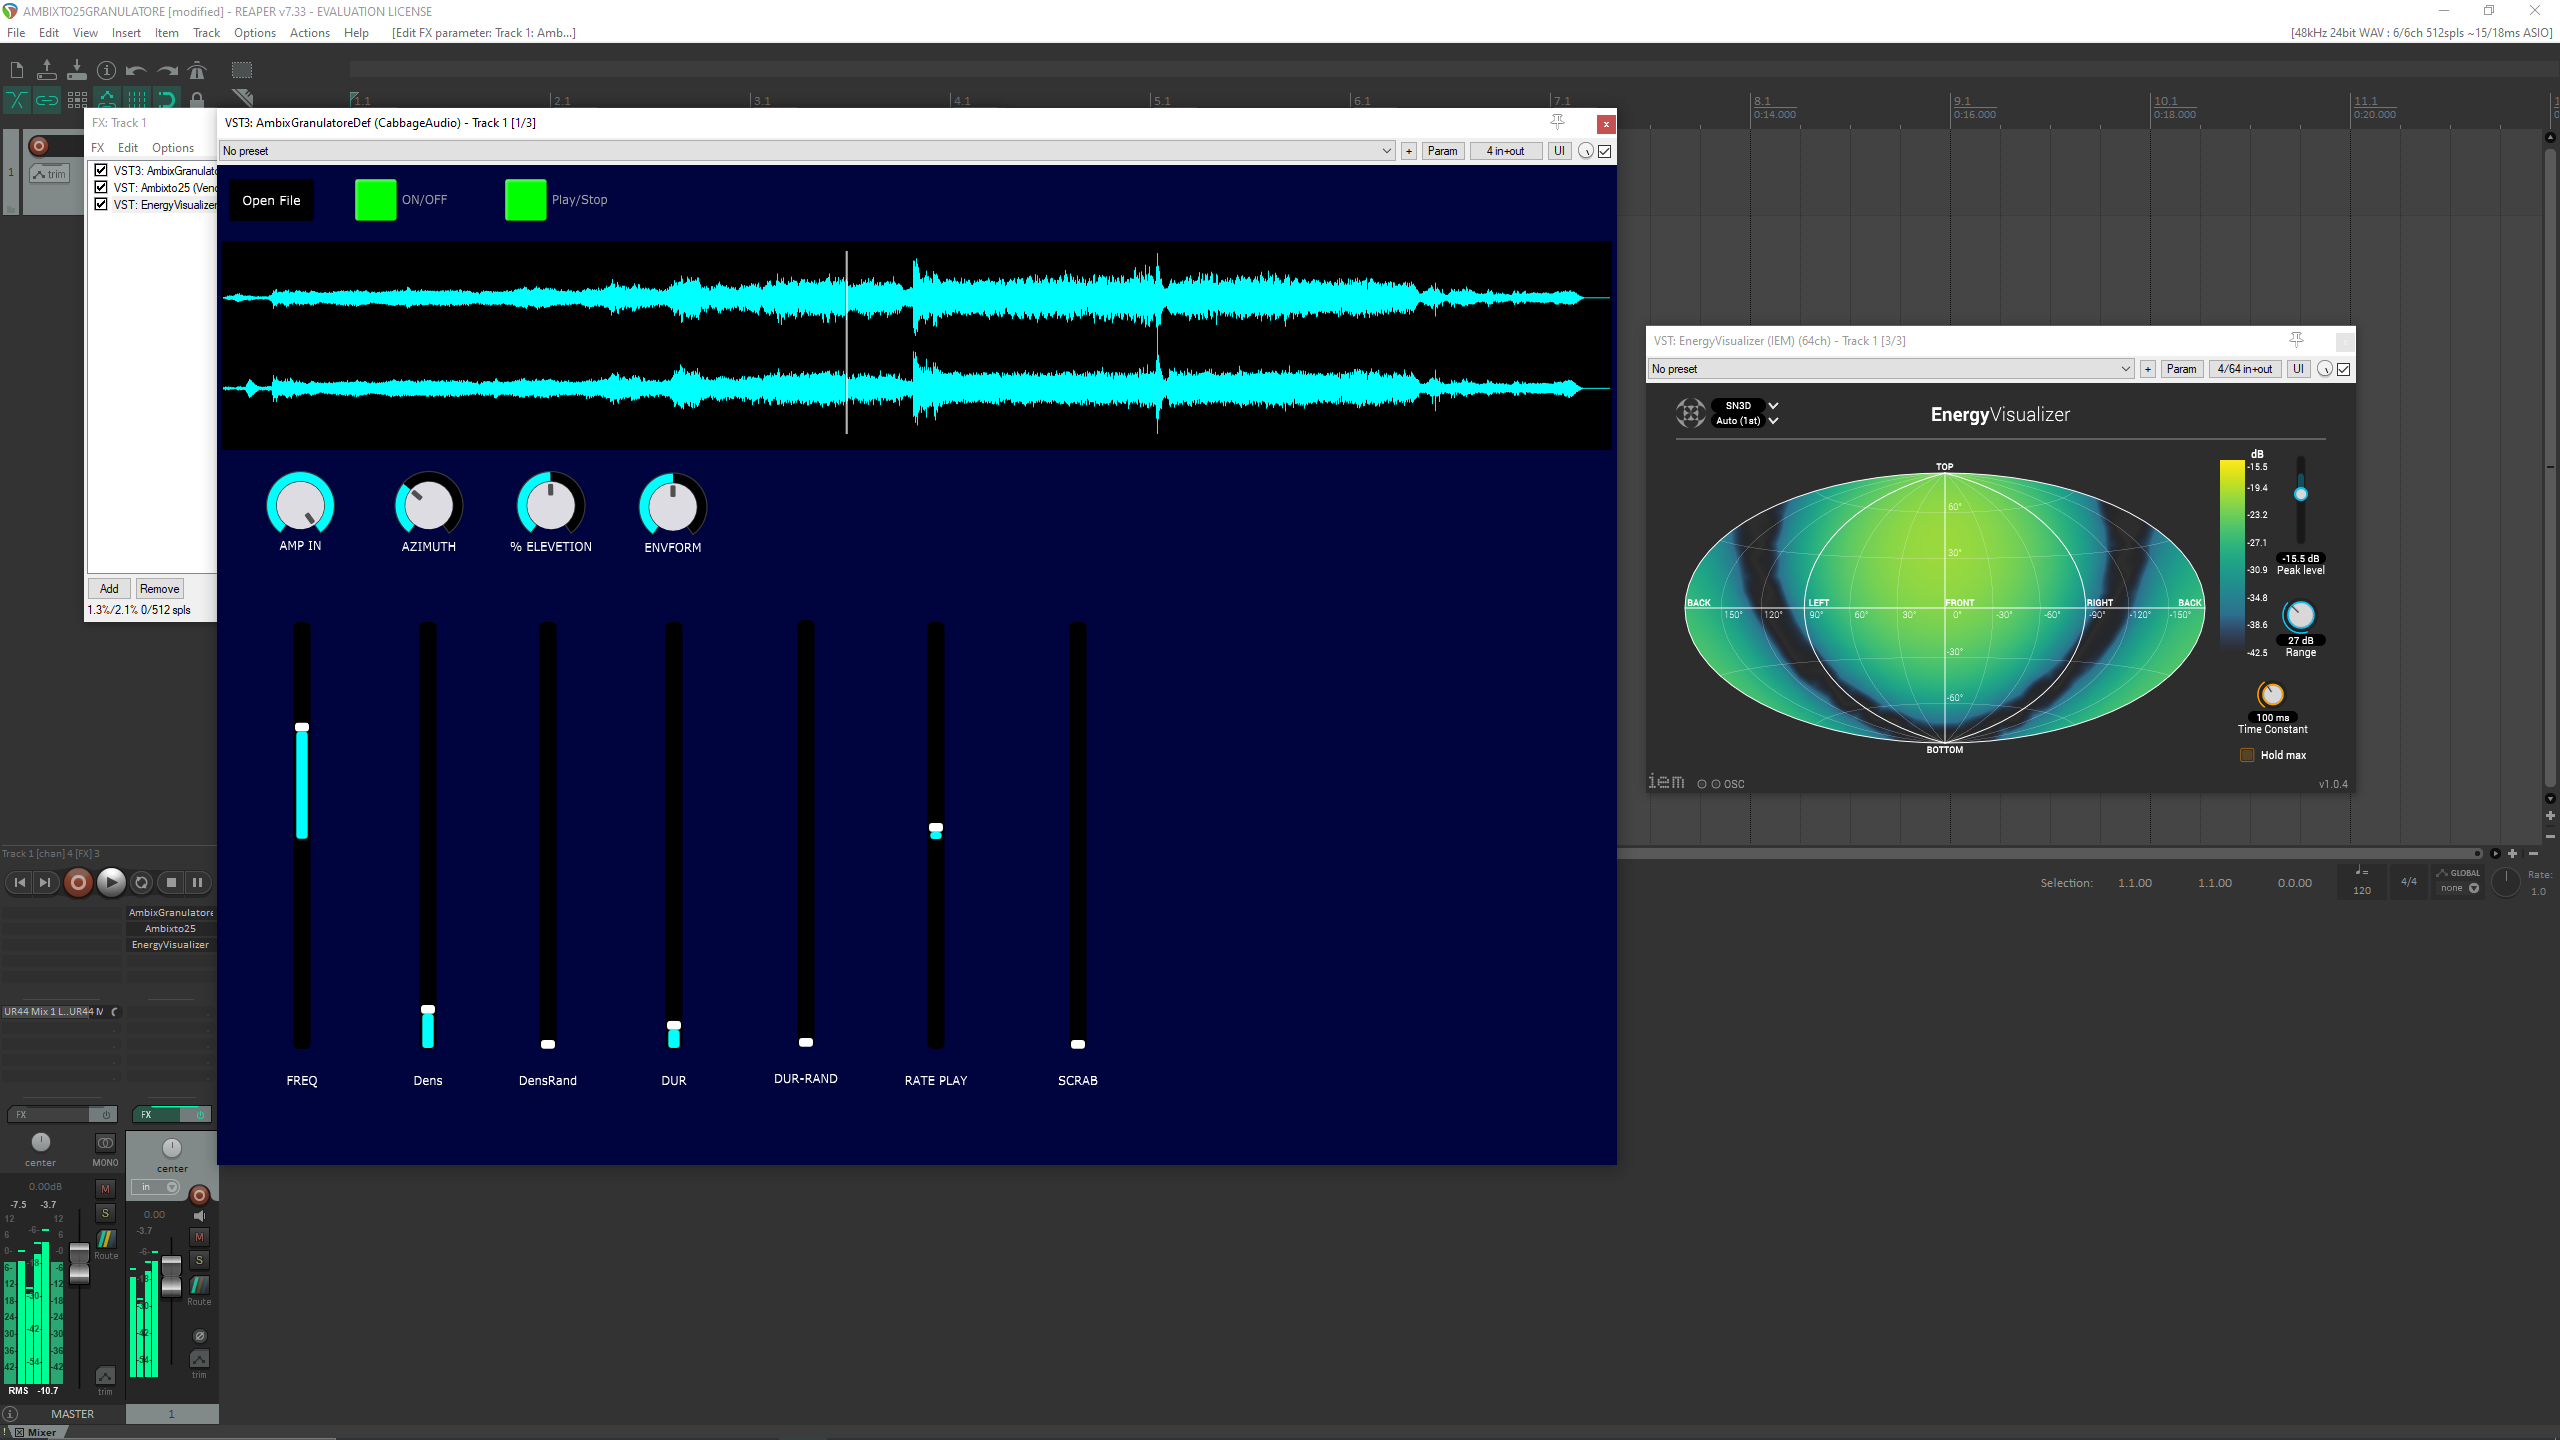
\includegraphics[width=0.8\textwidth]{img/AZIMUTH/Screenshot (4).png}}
    \caption{Visualizzazione dell'effetto ciambella in \foa}
    \label{fig:donut_effect}
\end{figure}

\subsubsection{Cause Tecniche}

L'origine di questo artefatto risiede nella natura matematica della codifica \foa:

\begin{itemize}
    \item Utilizzo di sole quattro componenti per rappresentare l'intero campo sferico
    \item Impossibilità di concentrare energia uniformemente in tutte le direzioni
    \item Interferenze costruttive e distruttive tra le componenti X, Y, Z
\end{itemize}

\subsubsection{Strategie di Mitigazione}

In \granix, l'effetto ciambella può essere attenuato attraverso:

\begin{enumerate}
    \item \textbf{Aumento della densità granulare}: Maggiore sovrapposizione temporale
    \item \textbf{Incremento della durata dei grani}: Maggiore copertura temporale
    \item \textbf{Controllo attivo dell'elevation}: Sfruttamento ottimale della componente Z
    \item \textbf{Randomizzazione spaziale}: Distribuzione statistica dell'energia
\end{enumerate}

\chapter{Architettura di \granix}

\section{Panoramica del Sistema}

\granix\ è sviluppato utilizzando \csound\ come motore di sintesi audio e \cabbage\ per l'interfaccia grafica. Questa architettura garantisce potenza computazionale elevata, flessibilità nella programmazione e compatibilità cross-platform.

\section{Struttura degli Strumenti \csound}

Il codice è organizzato secondo una separazione funzionale in quattro strumenti principali:

\subsection{Instrument 100 - Controller Principale}

Lo strumento 100 funge da \textit{master controller}, gestendo:

\begin{itemize}
    \item Interfacciamento con i controlli GUI
    \item Coordinamento degli altri strumenti
    \item Gestione dello stato globale del sistema
    \item Attivazione/disattivazione del granulatore
\end{itemize}

\subsection{Instrument 99 - Caricatore File}

Responsabile della gestione del materiale audio sorgente:

\begin{itemize}
    \item Caricamento file audio in memoria
    \item Calcolo parametri del file (durata, frequenza di campionamento)
    \item Configurazione del display waveform
    \item Supporto formati mono e multicanale
\end{itemize}

\subsection{Instrument 1 - Engine di Playback}

Gestisce il motore di riproduzione e scheduling dei grani:

\begin{itemize}
    \item Controllo transport (play/stop/velocità)
    \item Generazione trigger temporali per i grani
    \item Gestione del playhead tramite oscillatori phasor
    \item Implementazione scrubbing e randomizzazione posizionale
\end{itemize}

\subsection{Instrument 2 - Generatore Grani}

Il core della sintesi granulare:

\begin{itemize}
    \item Creazione dei singoli grani audio
    \item Applicazione degli inviluppi dinamici
    \item Spazializzazione \ambisonics\ in tempo reale
    \item Output in formato \ambix
\end{itemize}

\section{Opcode Personalizzato AmbixFra}

Il cuore della spazializzazione è l'opcode personalizzato \texttt{AmbixFra}, che implementa l'encoding \ambisonics:

\begin{lstlisting}[caption={Implementazione opcode AmbixFra}, label={lst:ambixfra}]
opcode AmbixFra, aaaa, akk
    ; Input: segnale audio, azimuth, elevation
    aSig, kazi, kelev xin
    
    ; Conversione gradi in radianti
    kElevRad = (kelev / 180) * $M_PI
    kAziRad = (kazi / 180) * $M_PI

    ; Encoding secondo formato AmbiX
    a0 = aSig                                ; W*sqrt(2) (omnidirezionale)
    a1 = aSig * sin(kAziRad) * cos(kElevRad) ; Y (sinistra-destra)
    a2 = aSig * sin(kElevRad)                ; Z (alto-basso)
    a3 = aSig * cos(kAziRad) * cos(kElevRad) ; X (avanti-dietro)

    ; Output dei quattro canali AmbiX
    xout a0, a1, a2, a3
endop
\end{lstlisting}

\section{Algoritmi di Spazializzazione Dinamica}

\subsection{Azimuth Dinamico}

L'azimuth in \granix\ non è statico ma varia dinamicamente secondo la posizione nel buffer audio:

\begin{equation}
\theta_{output} = \theta_{user} + (\phi_{buffer} \times 360°)
\end{equation}

dove $\phi_{buffer}$ rappresenta la fase normalizzata (0-1) della posizione nel file.

\subsection{Elevation Correlata}

L'elevation combina randomizzazione, densità granulare e ampiezza del segnale:

\begin{equation}
\phi_{output} = (rnd(180°) - 90°) \times \rho_{density} \times \alpha_{control} \times A_{signal}
\end{equation}

dove:
\begin{itemize}
    \item $rnd(180°)$: Valore random tra 0° e 180°
    \item $\rho_{density}$: Fattore di densità normalizzato
    \item $\alpha_{control}$: Controllo percentuale utente (0-1)
    \item $A_{signal}$: Ampiezza istantanea del segnale
\end{itemize}

\chapter{Interfaccia Utente}

\section{Design e Filosofia Visiva}

L'interfaccia di \granix\ è progettata seguendo principi di ergonomia cognitiva e estetica minimalista. La palette cromatica riflette l'identità del software e garantisce leggibilità ottimale anche in condizioni di luce variabile.

\begin{figure}[H]
    \centering
    % Placeholder per screenshot interfaccia completa
    \fbox{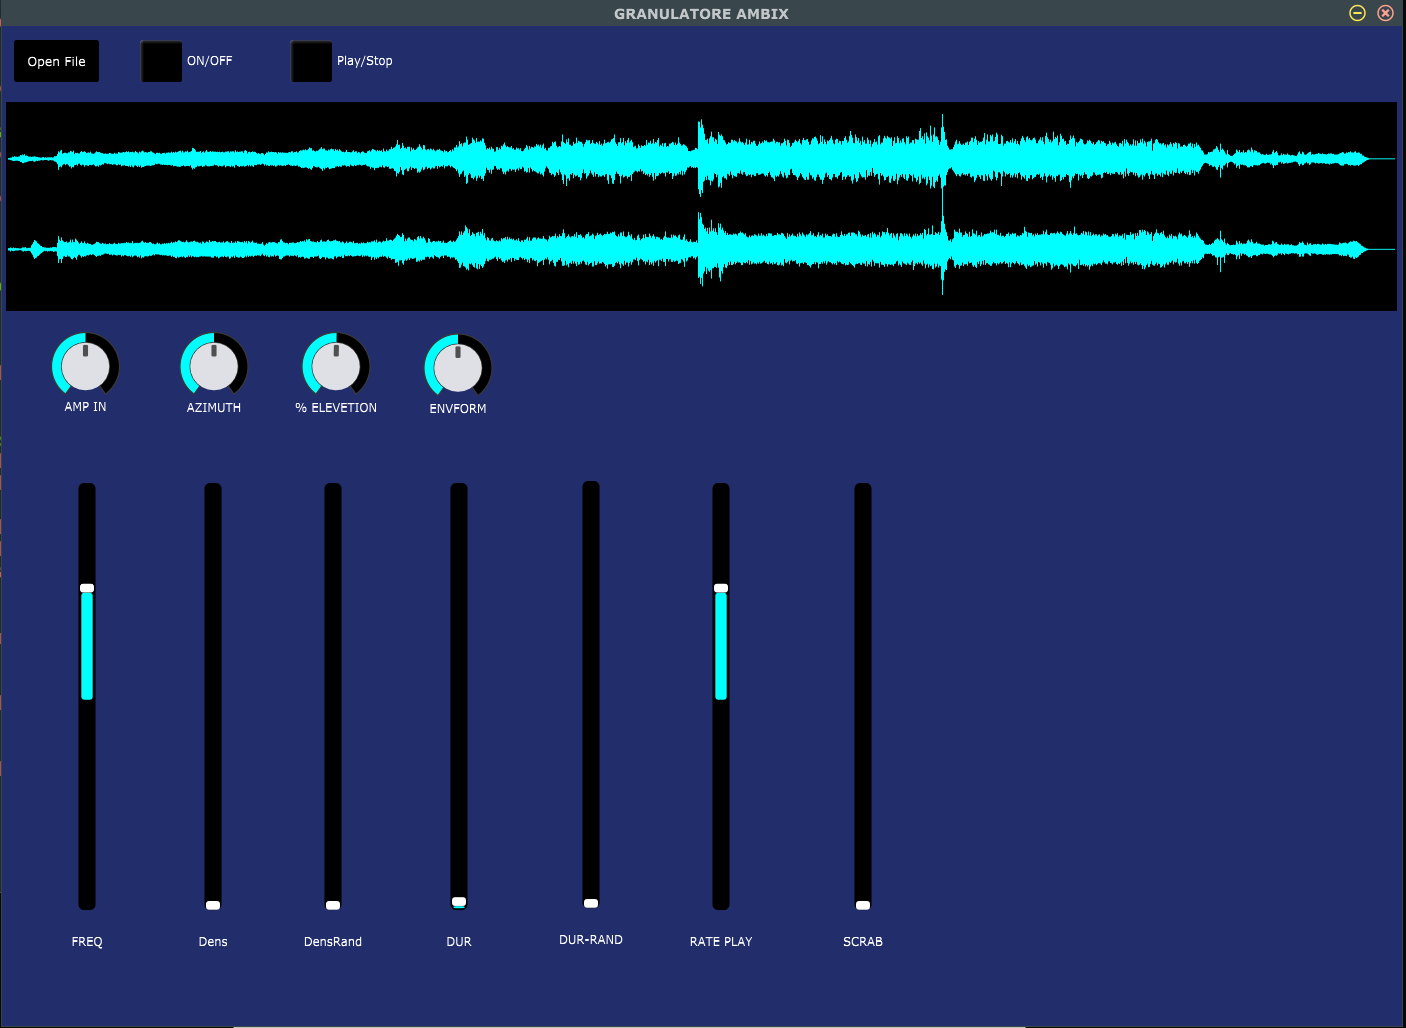
\includegraphics[width=\textwidth]{img/GUI/GUI NUOVA Buff pieno.PNG}}
    \caption{Interfaccia completa di \granix\ con file audio caricato}
    \label{fig:interface_complete}
\end{figure}

\subsection{Palette Cromatica}

\begin{table}[H]
    \centering
    \caption{Palette cromatica dell'interfaccia}
    \label{tab:color_palette}
    \begin{tabular}{@{}llp{5cm}@{}}
        \toprule
        \textbf{Elemento} & \textbf{Colore (RGB)} & \textbf{Utilizzo} \\
        \midrule
        Sfondo principale & (0, 10, 160) & Background generale, riduce affaticamento \\
        Controlli attivi & (0, 255, 255) & Slider, indicatori, cursore waveform \\
        Testo e etichette & (255, 255, 255) & Leggibilità massima su sfondo scuro \\
        Pulsanti attivi & Verde acido & Feedback stato ON/OFF, Play/Stop \\
        \bottomrule
    \end{tabular}
\end{table}

\section{Layout e Organizzazione}

\subsection{Sezione Transport}

La barra superiore contiene i controlli essenziali per l'operatività di base:

\begin{figure}[H]
    \centering
    % Placeholder per sezione transport
    \fbox{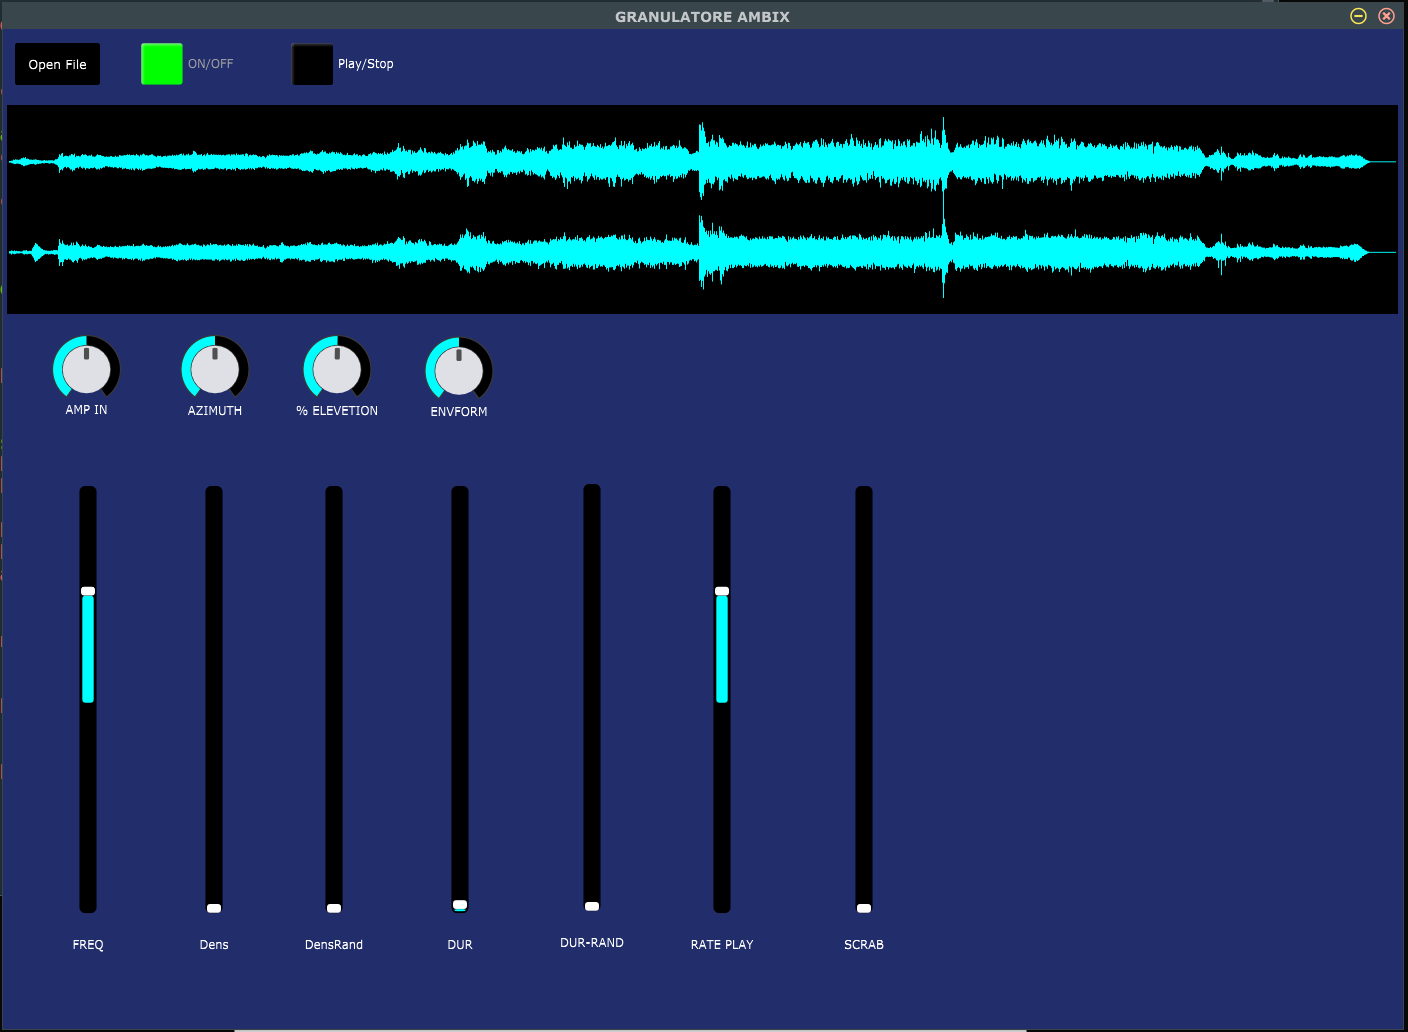
\includegraphics[width=0.8\textwidth]{img/GUI/GUI NUOVA ON .PNG}}
    \caption{Sezione transport con controlli di base}
    \label{fig:transport}
\end{figure}

\begin{itemize}
    \item \textbf{Open File}: Apertura file audio (formati supportati: WAV, AIFF, FLAC)
    \item \textbf{ON/OFF}: Attivazione granulatore (verde acido quando attivo)
    \item \textbf{Play/Stop}: Controllo playback (verde acido durante riproduzione)
\end{itemize}

\subsection{Display Waveform}

Il display centrale mostra la rappresentazione visiva del file audio caricato:

\begin{figure}[H]
    \centering
    % Placeholder per waveform display
    \fbox{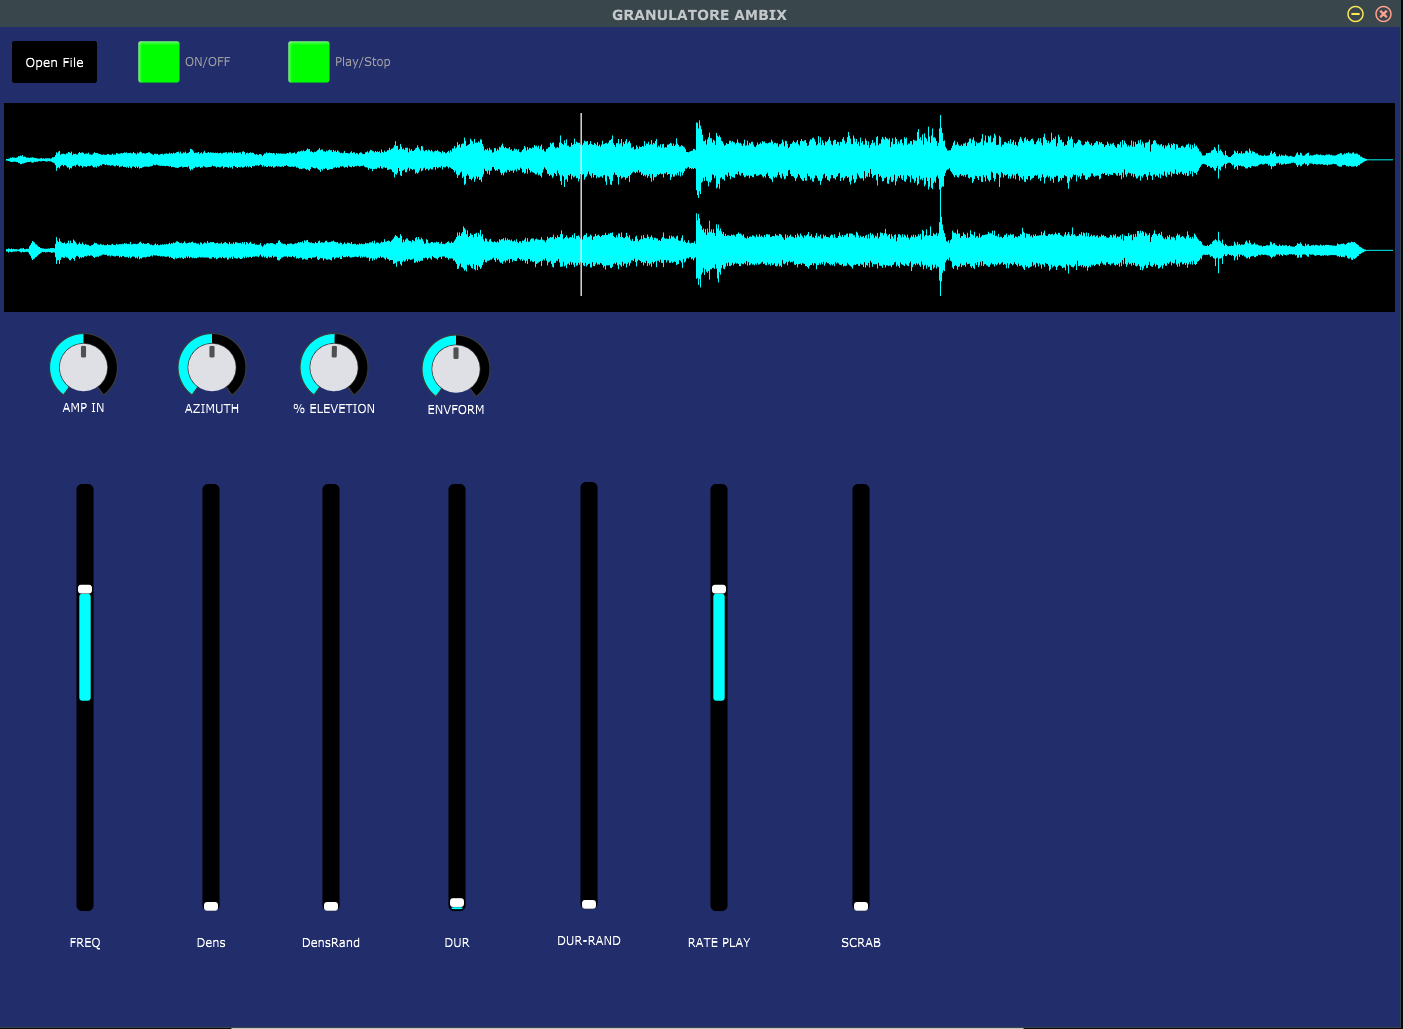
\includegraphics[width=\textwidth]{img/GUI/GUI NUOVA PLAY.PNG}}
    \caption{Display waveform con cursore di posizione}
    \label{fig:waveform}
\end{figure}

Caratteristiche del display:
\begin{itemize}
    \item Waveform in turchese su sfondo nero
    \item Cursore bianco verticale indica posizione corrente
    \item Scala temporale automatica in base alla durata del file
    \item Supporto file stereo (canali separati)
\end{itemize}

\subsection{Controlli Ambisonici}

La sezione superiore dei controlli gestisce i parametri spaziali:

\begin{itemize}
    \item \textbf{AMP IN}: Controllo amplificazione generale
    \item \textbf{AZIMUTH}: Posizionamento orizzontale (-180° a +180°)
    \item \textbf{\% ELEVATION}: Intensità movimento verticale (0-100\%)
    \item \textbf{ENVFORM}: Forma inviluppo grani (0.001-0.999)
\end{itemize}

\subsection{Controlli Granulari}

La sezione inferiore raggruppa i parametri principali della granulazione:

\section{Stati dell'Interfaccia}

\subsection{Stato Iniziale}

All'avvio, \granix\ presenta uno stato neutro:

\begin{figure}[H]
    \centering
    % Placeholder per interfaccia iniziale
    \fbox{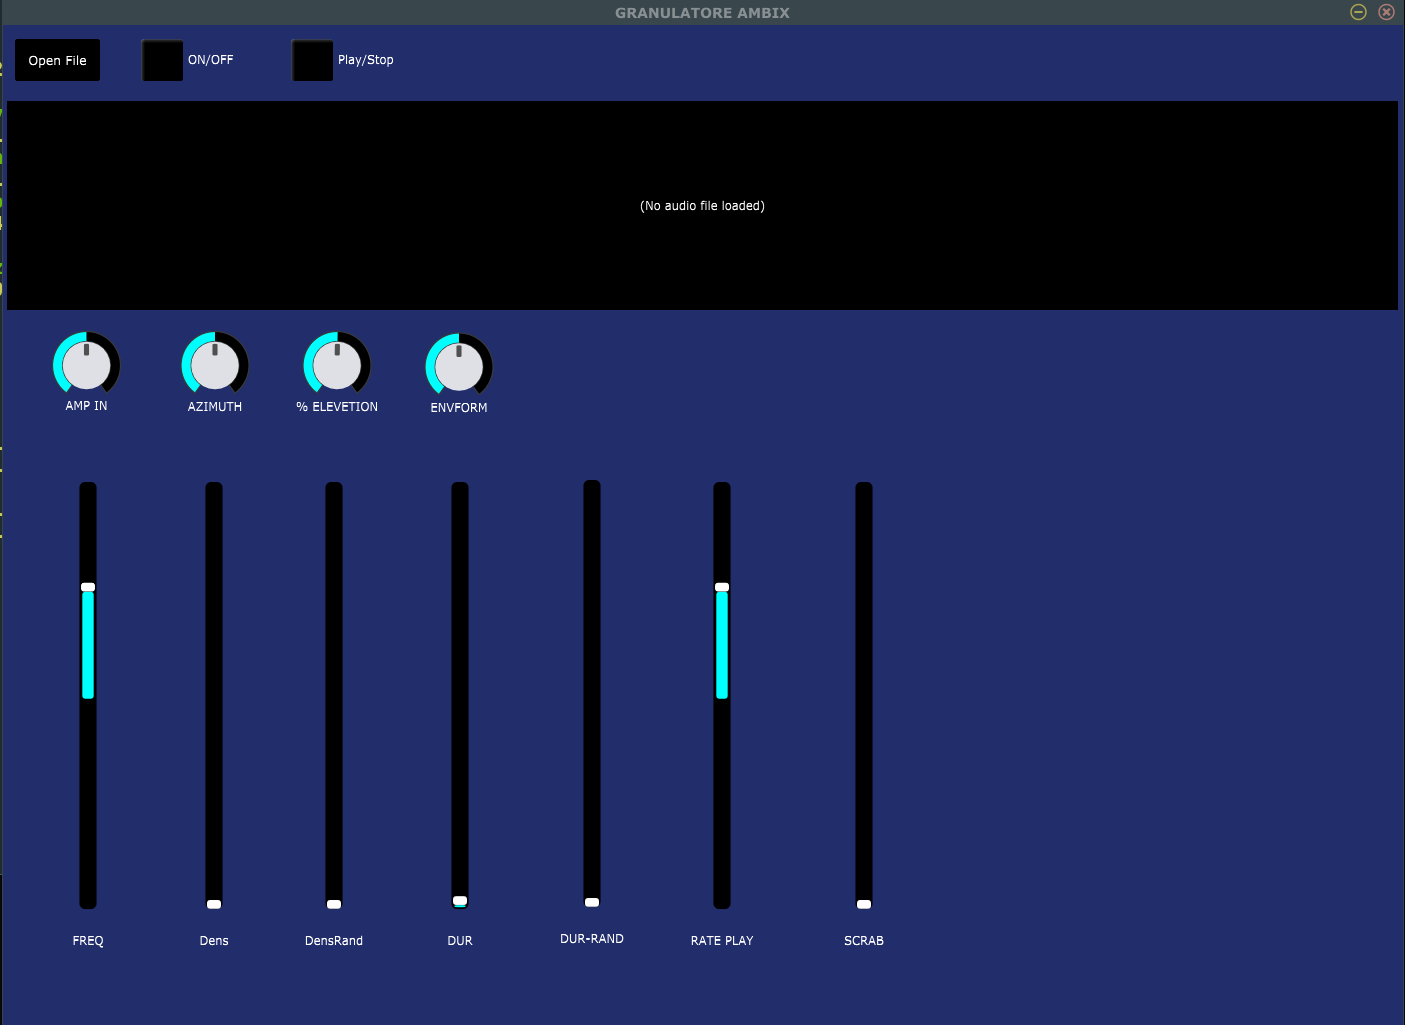
\includegraphics[width=0.8\textwidth]{img/GUI/GUI Nuova vuota.PNG}}
    \caption{Interfaccia allo stato iniziale}
    \label{fig:interface_initial}
\end{figure}

\begin{itemize}
    \item Buffer vuoto con messaggio "(No audio file loaded)"
    \item Tutti i controlli in posizione di default
    \item Pulsanti transport in stato inattivo
\end{itemize}

\subsection{File Caricato}

Dopo il caricamento di un file audio:

\begin{figure}[H]
    \centering
    % Placeholder per interfaccia con file
    \fbox{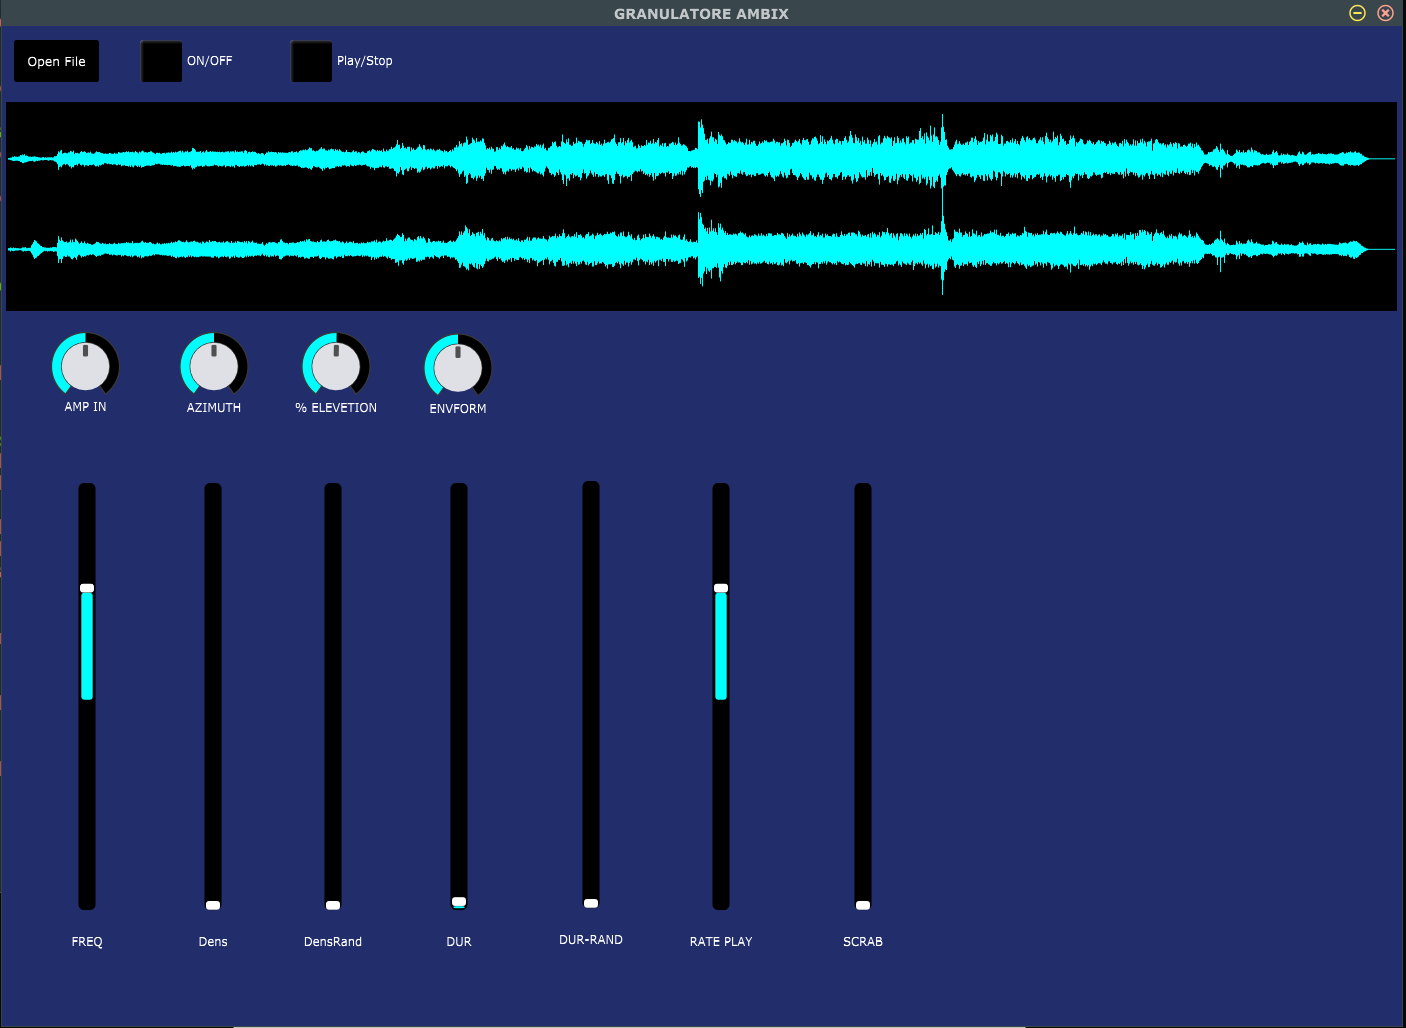
\includegraphics[width=0.8\textwidth]{img/GUI/GUI NUOVA Buff pieno.PNG}}
    \caption{Interfaccia con file audio caricato}
    \label{fig:interface_loaded}
\end{figure}

\begin{itemize}
    \item Waveform visibile nel buffer
    \item Cursore di posizione disponibile
    \item Controlli attivati e responsivi
\end{itemize}

\subsection{Granulatore Attivo}

Con il granulatore attivato:

\begin{figure}[H]
    \centering
    % Placeholder per granulatore attivo
    \fbox{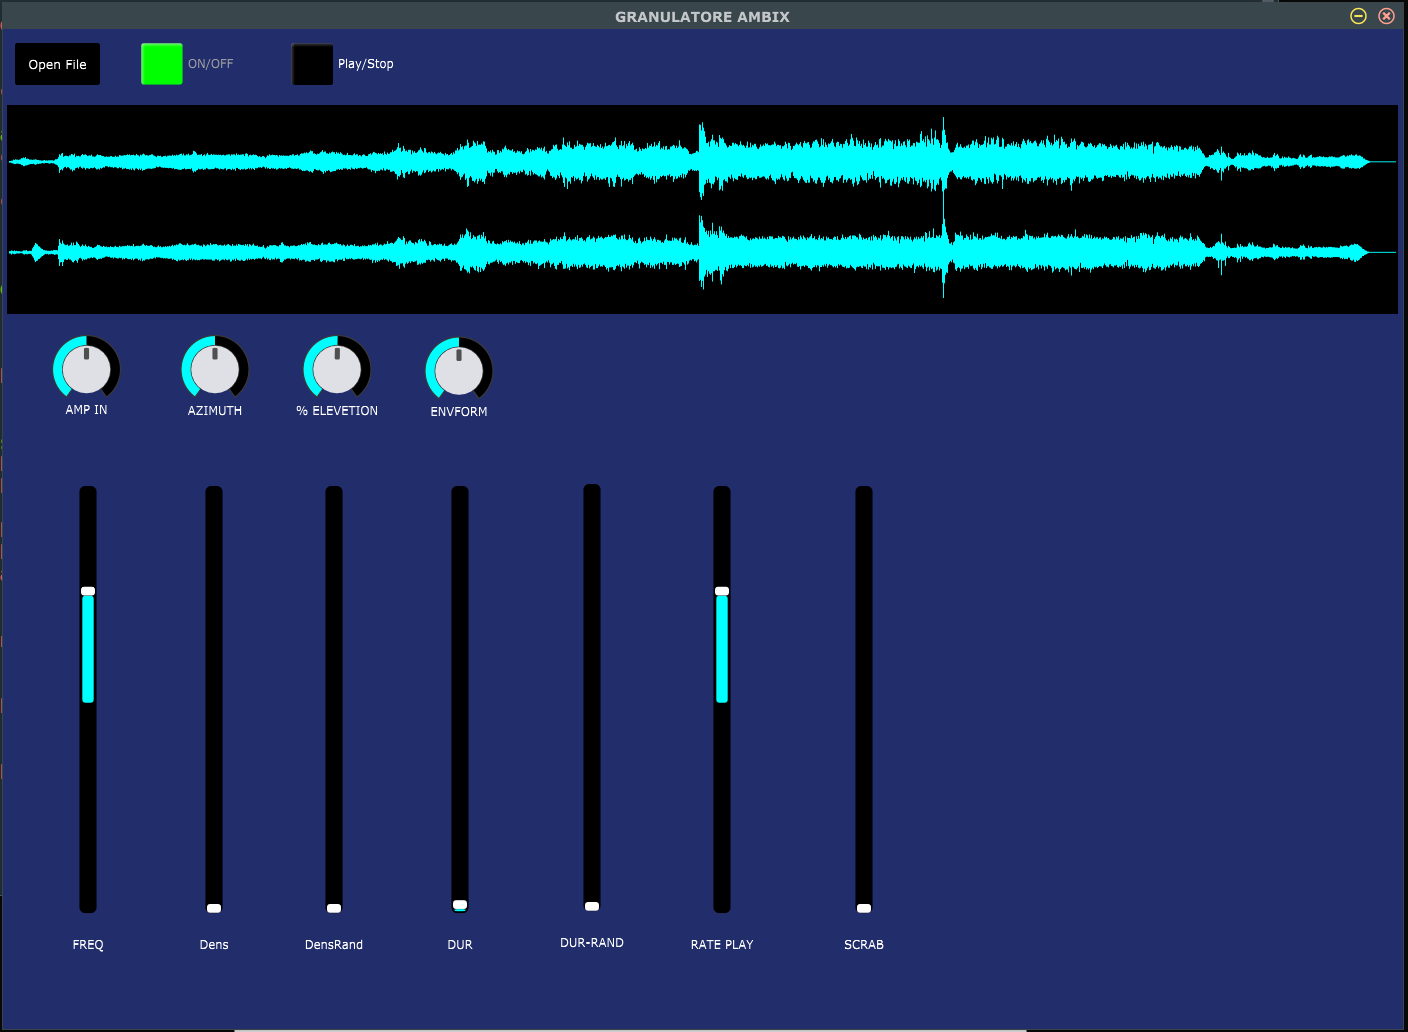
\includegraphics[width=0.8\textwidth]{img/GUI/GUI NUOVA ON .PNG}}
    \caption{Granulatore in stato attivo}
    \label{fig:interface_active}
\end{figure}

\begin{itemize}
    \item Pulsante ON/OFF in verde acido
    \item Granulazione attiva anche con playback fermo
    \item Feedback visuale sui controlli attivi
\end{itemize}

\subsection{Playback in Corso}

Durante la riproduzione:

\begin{figure}[H]
    \centering
    % Placeholder per playback attivo
    \fbox{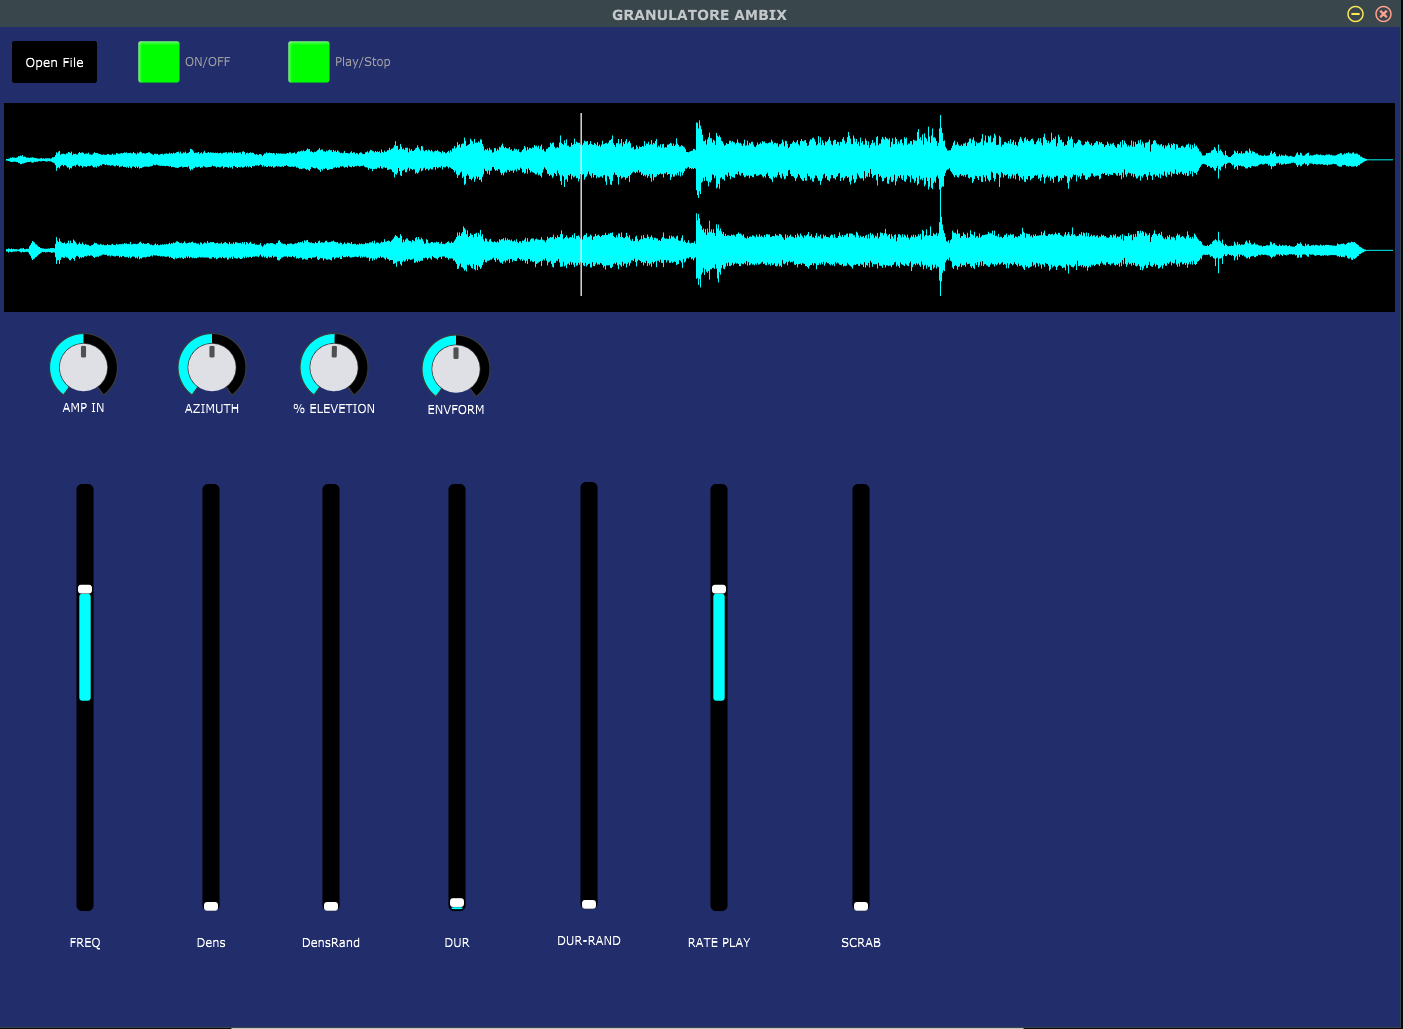
\includegraphics[width=0.8\textwidth]{img/GUI/GUI NUOVA PLAY.PNG}}
    \caption{Interfaccia durante il playback}
    \label{fig:interface_playing}
\end{figure}

\begin{itemize}
    \item Pulsante Play/Stop in verde acido
    \item Cursore bianco in movimento nel buffer
    \item Azimuth ed elevation dinamici attivi
\end{itemize}

\chapter{Controlli e Parametri}

\section{Controlli di Transport}

\subsection{Open File}

Il controllo \textbf{Open File} permette la selezione del materiale audio sorgente per la granulazione.

\begin{parambox}{Specifiche Open File}
\textbf{Formati supportati:} WAV, AIFF, FLAC, AU \\
\textbf{Risoluzione:} 16/24/32 bit \\
\textbf{Frequenze di campionamento:} 22.05, 44.1, 48, 88.2, 96 kHz \\
\textbf{Canali:} Mono, Stereo (downmix automatico) \\
\textbf{Durata massima:} Limitata dalla memoria RAM disponibile
\end{parambox}

\subsection{ON/OFF}

Controllo principale per l'attivazione del granulatore.

\begin{parambox}{Comportamento ON/OFF}
\textbf{Stato OFF:} Granulatore disattivato, nessun output audio \\
\textbf{Stato ON:} Granulatore attivo, elaborazione in tempo reale \\
\textbf{Indicazione visiva:} Verde acido quando attivo \\
\textbf{Nota:} La granulazione funziona anche con playback fermo
\end{parambox}

\subsection{Play/Stop}

Controllo del playback del file audio sorgente.

\begin{parambox}{Modalità Playback}
\textbf{Stop:} Posizione congelata nel buffer \\
\textbf{Play:} Avanzamento secondo Rate Play \\
\textbf{Indicazione:} Verde acido durante riproduzione \\
\textbf{Interazione:} Combinato con Rate Play per controllo direzionale
\end{parambox}

\section{Controlli Granulari}

\subsection{FREQ - Frequenza di Lettura}

Controlla la velocità di riproduzione dei grani, influenzando il pitch risultante.

\begin{table}[H]
    \centering
    \caption{Valori FREQ e risultati sonori}
    \label{tab:freq_values}
    \begin{tabular}{@{}ccp{6cm}@{}}
        \toprule
        \textbf{Valore} & \textbf{Trasposizione} & \textbf{Effetto} \\
        \midrule
        2.0 & +1 ottava & Pitch molto acuto, velocità doppia \\
        1.5 & +quinta & Pitch aumentato, carattere brillante \\
        1.0 & Originale & Nessuna trasposizione \\
        0.5 & -1 ottava & Pitch grave, velocità dimezzata \\
        0.25 & -2 ottave & Pitch molto grave, effetto drammatico \\
        \bottomrule
    \end{tabular}
\end{table}

\begin{esempio}{Pitch Shifting Creativo}
\textbf{Impostazione:} FREQ = 1.7, DENS = 100, DUR = 30ms \\
\textbf{Risultato:} Trasposizione di circa +9 semitoni con texture granulare densa \\
\textbf{Applicazione:} Creazione di harmonizer naturali su materiale percussivo
\end{exemplo}

\subsection{DENS - Densità Granulare}

Determina il numero di grani generati per secondo, influenzando la continuità percettiva.

\begin{table}[H]
    \centering
    \caption{Categorie di densità granulare}
    \label{tab:density_categories}
    \begin{tabular}{@{}cp{3cm}p{6cm}@{}}
        \toprule
        \textbf{Range} & \textbf{Categoria} & \textbf{Caratteristiche Percettive} \\
        \midrule
        1-5 grani/sec & Ritmica & Eventi discreti, pattern percettibili \\
        10-30 grani/sec & Texture & Granularità evidente, superficie rugosa \\
        50-100 grani/sec & Flusso & Continuità con carattere granulare \\
        200+ grani/sec & Sintesi & Flusso continuo, colorazione timbrica \\
        \bottomrule
    \end{tabular}
\end{table}

\subsection{DENSRAND - Randomizzazione Densità}

Introduce variabilità temporale nella generazione dei grani.

\begin{parambox}{Effetti DENSRAND}
\textbf{Valore 0.0:} Generazione perfettamente regolare \\
\textbf{Valore 0.3:} Leggera irregolarità, effetto "umano" \\
\textbf{Valore 0.7:} Forte irregolarità, carattere caotico \\
\textbf{Valore 1.0:} Massima randomizzazione, eventi sparsi
\end{parambox}

\subsection{DUR - Durata Grani}

Controlla l'estensione temporale di ogni singolo grano.

\begin{itemize}
    \item \textbf{Grani corti (1-20ms):} Effetti percussivi, attacchi definiti
    \item \textbf{Grani medi (30-80ms):} Bilanciamento tra articolazione e fluidità
    \item \textbf{Grani lunghi (100-500ms):} Texture scorrevoli, sovrapposizioni evidenti
\end{itemize}

\subsection{DURRAND - Randomizzazione Durata}

Varia casualmente la durata dei grani per aumentare la complessità timbrica.

\begin{exemplo}{Texture Complessa}
\textbf{Impostazione:} DUR = 60ms, DURRAND = 0.8 \\
\textbf{Risultato:} Grani di durata variabile tra ~12ms e ~108ms \\
\textbf{Effetto:} Superficie granulare irregolare, ricchezza timbrica elevata
\end{exemplo}

\subsection{ENVFORM - Forma Inviluppo}

Modifica il rapporto tra attacco e rilascio nell'inviluppo triangolare dei grani.

\begin{table}[H]
    \centering
    \caption{Valori ENVFORM e caratteristiche}
    \label{tab:envform_values}
    \begin{tabular}{@{}cp{4cm}p{5cm}@{}}
        \toprule
        \textbf{Valore} & \textbf{Caratteristica} & \textbf{Applicazione} \\
        \midrule
        0.1 & Attacco veloce, rilascio lungo & Effetti percussivi morbidi \\
        0.5 & Forma simmetrica & Utilizzo generale, bilanciato \\
        0.9 & Attacco lungo, rilascio veloce & Effetti di fade-in naturali \\
        \bottomrule
    \end{tabular}
\end{table}

\section{Controlli di Riproduzione}

\subsection{RATE PLAY - Velocità Riproduzione}

Determina velocità e direzione del playback nel buffer audio.

\begin{parambox}{Range RATE PLAY}
\textbf{Valori positivi:} Riproduzione in avanti \\
\textbf{Valore 0:} Posizione congelata \\
\textbf{Valori negativi:} Riproduzione all'indietro (reverse) \\
\textbf{Range:} -2.0 a +2.0 \\
\textbf{Valore 1.0:} Velocità normale del file originale
\end{parambox}

\begin{esempio}{Effetto Reverse Granulare}
\textbf{Impostazione:} RATE PLAY = -0.5, FREQ = 0.8, DENS = 80 \\
\textbf{Risultato:} Reverse lento con pitch leggermente abbassato \\
\textbf{Carattere:} Effetto "rewind" granulare, molto espressivo
\end{esempio}

\subsection{SCRAB - Posizione Random}

Introduce oscillazioni casuali nel puntatore di lettura del buffer.


\begin{itemize}
    \item \textbf{Valore 0.0:} Lettura lineare senza deviazioni
    \item \textbf{Valore 0.3:} Leggere oscillazioni, effetto "tape flutter"
    \item \textbf{Valore 0.8:} Forti salti posizionali, frammentazione del materiale
    \item \textbf{Valore 1.0:} Lettura completamente randomizzata
\end{itemize}

\section{Controlli Ambisonici}

\subsection{AZIMUTH - Posizionamento Orizzontale}

Controlla la posizione base nell'asse orizzontale, con rotazione automatica correlata alla posizione nel buffer.

\begin{parambox}{Funzionamento AZIMUTH}
\textbf{Formula:} $\theta_{finale} = \theta_{controllo} + (\phi_{buffer} \times 360°)$ \\
\textbf{Effetto:} Rotazione continua durante il playback \\
\textbf{Controllo utente:} Offset della posizione di partenza \\
\textbf{Range:} -180° a +180°
\end{parambox}

\subsection{\% ELEVATION - Controllo Elevazione}

Modula l'intensità del movimento verticale automatico.

\begin{table}[H]
    \centering
    \caption{Effetti della percentuale di elevation}
    \label{tab:elevation_effects}
    \begin{tabular}{@{}cp{4cm}p{5cm}@{}}
        \toprule
        \textbf{Percentuale} & \textbf{Comportamento} & \textbf{Risultato Percettivo} \\
        \midrule
        0\% & Elevation disattivata & Movimento solo orizzontale \\
        25\% & Elevation moderata & Leggero movimento 3D \\
        50\% & Elevation bilanciata & Movimento spaziale evidente \\
        75\% & Elevation pronunciata & Forte dinamismo verticale \\
        100\% & Elevation massima & Movimento spaziale estremo \\
        \bottomrule
    \end{tabular}
\end{table}

\subsection{AMP IN - Amplificazione Ingresso}

Controllo del volume generale dell'output granulare.

\begin{parambox}{Gestione AMP IN}
\textbf{Range:} 0.0 a 1.0 \\
\textbf{Curva:} Lineare \\
\textbf{Posizione ottimale:} 0.7-0.8 per la maggior parte del materiale \\
\textbf{Attenzione:} Valori elevati possono causare clipping con alta densità
\end{parambox}

\chapter{Tecniche Creative e Preset}

\subsection{Ambient Ethereal}

Creazione di atmosfere sospese e immersive.

\begin{exemplo}{Preset Ambient Ethereal}
\textbf{Parametri:}
\begin{itemize}
    \item FREQ: 0.5 (una ottava sotto)
    \item DENS: 45 grani/sec
    \item DENSRAND: 0.4
    \item DUR: 120ms
    \item DURRAND: 0.6
    \item RATE PLAY: 0.1 (molto lento)
    \item SCRAB: 0.2
    \item AZIMUTH: 0° (fronte)
    \item \% ELEVATION: 85\%
    \item ENVFORM: 0.3
\end{itemize}
\textbf{Risultato:} Nuvola granulare grave con movimento spaziale pronunciato, ideale per introduzioni o transizioni atmosferiche.
\end{exemplo}

\subsection{Rhythmic Pulse}

Generazione di pattern ritmici spazializzati.

\begin{exemplo}{Preset Rhythmic Pulse}
\textbf{Parametri:}
\begin{itemize}
    \item FREQ: 1.2 (leggermente acuto)
    \item DENS: 6 grani/sec
    \item DENSRAND: 0.15
    \item DUR: 40ms
    \item DURRAND: 0.25
    \item RATE PLAY: 0 (fermo)
    \item SCRAB: 0.7
    \item AZIMUTH: variazione manuale
    \item \% ELEVATION: 30\%
    \item ENVFORM: 0.8
\end{itemize}
\textbf{Risultato:} Pattern ritmico con salti casuali nel materiale e controllo espressivo dell'azimuth.
\end{exemplo}

\subsection{Spectral Morphing}

Trasformazioni timbriche continue attraverso pitch shifting dinamico.

\begin{exemplo}{Preset Spectral Morphing}
\textbf{Parametri:}
\begin{itemize}
    \item FREQ: 1.7 (settima maggiore sopra)
    \item DENS: 180 grani/sec
    \item DENSRAND: 0.1
    \item DUR: 25ms
    \item DURRAND: 0.3
    \item RATE PLAY: 0.4
    \item SCRAB: 0.1
    \item AZIMUTH: 45°
    \item \% ELEVATION: 60\%
    \item ENVFORM: 0.5
\end{itemize}
\textbf{Risultato:} Pitch shifting continuo con texture granulare fine e movimento spaziale controllato.
\end{exemplo}

\subsection{Chaos Cloud}

Texture caotica con massima randomizzazione.

\begin{exemplo}{Preset Chaos Cloud}
\textbf{Parametri:}
\begin{itemize}
    \item FREQ: automazione random (0.3-2.1)
    \item DENS: 250 grani/sec
    \item DENSRAND: 0.9
    \item DUR: 35ms
    \item DURRAND: 0.95
    \item RATE PLAY: 0.6
    \item SCRAB: 0.85
    \item AZIMUTH: automazione circolare
    \item \% ELEVATION: 100\%
    \item ENVFORM: 0.4
\end{itemize}
\textbf{Risultato:} Nuvola granulare caotica con massima imprevedibilità spaziale e timbrica.
\end{esempio}

\subsection{Reverse Wash}

Effetto di lavaggio sonoro all'indietro.

\begin{esempio}{Preset Reverse Wash}
\textbf{Parametri:}
\begin{itemize}
    \item FREQ: 0.75
    \item DENS: 120 grani/sec
    \item DENSRAND: 0.5
    \item DUR: 85ms
    \item DURRAND: 0.7
    \item RATE PLAY: -0.3 (reverse lento)
    \item SCRAB: 0.4
    \item AZIMUTH: -90° (destra)
    \item \% ELEVATION: 75\%
    \item ENVFORM: 0.2
\end{itemize}
\textbf{Risultato:} Effetto wash con movimento all'indietro, texture avvolgente con forte carattere spaziale.
\end{esempio}


\chapter{Workflow di Produzione}

\section{Preparazione del Materiale}

\subsection{Selezione del Materiale Sorgente}

La scelta del materiale audio influenza drasticamente i risultati ottenibili:

\begin{table}[H]
    \centering
    \caption{Caratteristiche del materiale sorgente e risultati}
    \label{tab:source_material}
    \begin{tabular}{@{}p{3cm}p{4cm}p{6cm}@{}}
        \toprule
        \textbf{Tipo Materiale} & \textbf{Caratteristiche} & \textbf{Risultati Granulari} \\
        \midrule
        Materiale percussivo & Attacchi definiti, spettro ricco & Texture ritmiche, effetti glitch \\
        Materiale sustain & Evoluzione lenta, timbro stabile & Pad atmosferici, morphing continuo \\
        Materiale vocale & Formanti, dinamica espressiva & Texture organiche, effetti parlati \\
        Materiale sintetico & Spettro controllato & Risultati prevedibili, purezza timbrica \\
        Field recordings & Complessità spettrale & Texture realistiche, ambienti sonori \\
        \bottomrule
    \end{tabular}
\end{table}

\subsection{Pre-processing Consigliato}

Prima del caricamento in \granix, alcuni processamenti possono migliorare i risultati:

\begin{enumerate}
    \item \textbf{Normalizzazione}: Ottimizzazione del range dinamico
    \item \textbf{EQ correttivo}: Rimozione di frequenze problematiche
    \item \textbf{Compressione leggera}: Controllo dei picchi eccessivi
    \item \textbf{De-clicking}: Rimozione di artefatti digitali
\end{enumerate}

\section{Metodologie di Registrazione}

\subsection{Setup di Monitoraggio \ambisonics}

Per un monitoraggio accurato dell'output \ambix:

\subsubsection{Configurazioni Altoparlanti}

\begin{itemize}
    \item \textbf{Quadrifonico}: 4 altoparlanti agli angoli (minimo per \foa)
    \item \textbf{Ottafonico}: 8 altoparlanti su circonferenza (ottimale per \foa)
    \item \textbf{Setup 3D}: Include altoparlanti elevation per full-sphere
\end{itemize}

\subsubsection{Decoder \ambisonics}

Selezione del decoder appropriato:

\begin{table}[H]
    \centering
    \caption{Decoder \ambisonics\ consigliati}
    \label{tab:ambisonic_decoders}
    \begin{tabular}{@{}lp{4cm}p{5cm}@{}}
        \toprule
        \textbf{Software} & \textbf{Caratteristiche} & \textbf{Applicazione} \\
        \midrule
        IEM AllRADecoder & Configurazione flessibile & Setup irregolari, ricerca \\
        Ambisonic Toolkit & Integrazione DAW & Produzione musicale \\
        SPARTA & Analisi real-time & Monitoraggio, debugging \\
        Blue Ripple O3A & Qualità professionale & Mastering, post-produzione \\
        \bottomrule
    \end{tabular}
\end{table}

\subsection{Tecniche di Registrazione}

\subsubsection{Registrazione Diretta}

Cattura dell'output \ambix\ in tempo reale:

\begin{enumerate}
    \item Configurazione DAW a 4 canali
    \item Routing diretto da \granix\ a tracce audio
    \item Registrazione simultanea di automazioni MIDI
    \item Backup dei preset utilizzati
\end{enumerate}

\subsubsection{Registrazione Layered}

Approccio per costruzioni complesse:

\begin{enumerate}
    \item Registrazione separata di ogni layer granulare
    \item Mixing in ambiente \ambisonics\ dedicato
    \item Post-processing su singoli layer
    \item Compositing finale con controllo spaziale
\end{enumerate}

\section{Post-Produzione \ambisonics}

\subsection{Editing e Montaggio}

\subsubsection{Strumenti Specifici}

Software specializzati per editing \ambisonics:

\begin{itemize}
    \item \textbf{Reaper} con plugin IEM: Soluzione economica e flessibile
    \item \textbf{Pro Tools} con Dolby Atmos: Standard industria
    \item \textbf{Pyramix} con Merging Technologies: Qualità professionale
    \item \textbf{Nuendo} con VST3 \ambisonics: Integrazione completa
\end{itemize}

\subsubsection{Tecniche di Editing}

\begin{itemize}
    \item \textbf{Crossfade spaziale}: Transizioni fluide tra posizioni
    \item \textbf{Automazione rotation}: Movimento dinamico post-registrazione
    \item \textbf{Distance control}: Simulazione profondità attraverso filtri
    \item \textbf{Diffusion control}: Controllo della larghezza della sorgente
\end{itemize}

\subsection{Mastering \ambisonics}

\subsubsection{Considerazioni Specifiche}

Il mastering in ambiente \ambisonics\ richiede attenzioni particolari:

\begin{enumerate}
    \item \textbf{Bilanciamento canali}: Verifica equilibrio W, X, Y, Z
    \item \textbf{Controllo correlazione}: Evitare cancellazioni di fase
    \item \textbf{Dynamic range}: Preservare dimensionalità spaziale
    \item \textbf{Translation check}: Verifica su diversi sistemi di riproduzione
\end{enumerate}

\subsubsection{Chain di Mastering}

Catena di processing consigliata:

\begin{enumerate}
    \item \textbf{Analisi spettrale 4-canali}: Identificazione problemi
    \item \textbf{EQ correttivo per canale}: Bilanciamento frequenziale
    \item \textbf{Compressore 4-canali linkato}: Controllo dinamica
    \item \textbf{Limiter trasparente}: Protezione da overload
    \item \textbf{Analisi finale}: Verifica conformità standard
\end{enumerate}

\chapter{Risoluzione Problemi e Ottimizzazione}

\section{Diagnostica Audio}

\subsection{Problemi di Output}

\subsubsection{Assenza di Segnale}

Procedura di diagnosi sistematica:


\begin{enumerate}
    \item \textbf{Verifica stato ON/OFF}: Controllo indicatore verde
    \item \textbf{Controllo AMP IN}: Valore maggiore di 0.1
    \item \textbf{Verifica file caricato}: Presenza waveform nel buffer
    \item \textbf{Test routing audio}: Controllo configurazione DAW
    \item \textbf{Verifica driver audio}: Controllo latenza e buffer size
\end{enumerate}

\subsubsection{Distorsione Audio}

Cause comuni e soluzioni:

\begin{table}[H]
    \centering
    \caption{Diagnosi distorsione audio}
    \label{tab:distortion_diagnosis}
    \begin{tabular}{@{}p{3cm}p{5cm}p{5cm}@{}}
        \toprule
        \textbf{Sintomo} & \textbf{Causa Probabile} & \textbf{Soluzione} \\
        \midrule
        Clipping digitale & AMP IN troppo alto & Ridurre AMP IN sotto 0.8 \\
        Artefatti granulari & Densità eccessiva & Limitare DENS sotto 300 \\
        Aliasing & File sorgente di bassa qualità & Utilizzare file 44.1kHz+ \\
        Glitch sporadici & Buffer audio troppo piccolo & Aumentare buffer a 256-512 \\
        Saturazione & Sovraccarico CPU & Ridurre densità e durata grani \\
        \bottomrule
    \end{tabular}
\end{table}

\subsection{Problemi di Spazializzazione}

\subsubsection{Spazializzazione Non Percepita}

Controlli da effettuare:

\begin{enumerate}
    \item \textbf{Routing 4-canali}: Verifica output AmbiX corretto
    \item \textbf{Decoder configurato}: Controllo decoder \ambisonics\ attivo
    \item \textbf{\% ELEVATION attiva}: Valore maggiore di 20\%
    \item \textbf{Movimento AZIMUTH}: Controllo rotazione durante playback
    \item \textbf{Sistema di ascolto}: Verifica configurazione altoparlanti
\end{enumerate}

\subsubsection{Effetto Ciambella Eccessivo}

Mitigazione dell'artefatto \foa:

\begin{exemplo}{Riduzione Effetto Ciambella}
\textbf{Strategia 1 - Densificazione:}
\begin{itemize}
    \item Aumentare DENS a 150+ grani/sec
    \item Incrementare DUR a 80+ ms
    \item Usare DURRAND = 0.6+
\end{itemize}

\textbf{Strategia 2 - Elevation ottimale:}
\begin{itemize}
    \item Impostare \% ELEVATION = 70-90\%
    \item Evitare elevation = 0\%
    \item Utilizzare DENSRAND = 0.4+
\end{itemize}
\end{exemplo}

\section{Ottimizzazione Performance}

\subsection{Configurazione Sistema}

\subsubsection{Impostazioni Audio Driver}

Parametri ottimali per diverse applicazioni:

\begin{table}[H]
    \centering
    \caption{Configurazioni audio consigliate}
    \label{tab:audio_settings}
    \begin{tabular}{@{}p{3cm}p{3cm}p{3cm}p{3cm}@{}}
        \toprule
        \textbf{Applicazione} & \textbf{Buffer Size} & \textbf{Sample Rate} & \textbf{Latenza Target} \\
        \midrule
        Performance Live & 128-256 samples & 44.1/48 kHz & <10ms \\
        Registrazione Studio & 512-1024 samples & 48/96 kHz & <20ms \\
        Composizione & 1024-2048 samples & 44.1/48 kHz & <40ms \\
        Rendering Offline & 2048+ samples & 96/192 kHz & Non critica \\
        \bottomrule
    \end{tabular}
\end{table}

\subsubsection{Gestione Memoria}

Ottimizzazione utilizzo RAM:

\begin{itemize}
    \item \textbf{File lunghi}: Considerare segmentazione
    \item \textbf{Qualità file}: Bilanciare qualità/memoria
    \item \textbf{Istanze multiple}: Monitorare utilizzo complessivo
    \item \textbf{Cleanup periodico}: Riavvio regolare per reset memoria
\end{itemize}

\subsection{Limits di Performance}

\subsubsection{CPU Usage Guidelines}

Linee guida per utilizzo CPU sostenibile:


\begin{table}[H]
    \centering
    \caption{Limiti consigliati per utilizzo CPU}
    \label{tab:cpu_limits}
    \begin{tabular}{@{}p{3cm}cp{6cm}@{}}
        \toprule
        \textbf{CPU Type} & \textbf{Max DENS} & \textbf{Note} \\
        \midrule
        Intel i5 (old gen) & 200 grani/sec & Limitare istanze simultanee \\
        Intel i7/i9 (new) & 500+ grani/sec & Performance eccellenti \\
        AMD Ryzen 5/7 & 400+ grani/sec & Ottima efficienza multi-core \\
        Apple M1/M2 & 600+ grani/sec & Architettura molto efficiente \\
        \bottomrule
    \end{tabular}
\end{table}

\section{Troubleshooting Avanzato}

\subsection{Problemi di Compatibilità}

\subsubsection{Host DAW}

Compatibilità con diverse DAW:

\begin{table}[H]
    \centering
    \caption{Compatibilità DAW e note specifiche}
    \label{tab:daw_compatibility}
    \begin{tabular}{@{}p{3cm}p{2cm}p{6cm}@{}}
        \toprule
        \textbf{DAW} & \textbf{Supporto} & \textbf{Note Specifiche} \\
        \midrule
        Reaper & Eccellente & Supporto nativo 4+ canali \\
        Logic Pro X & Buono & Configurare I/O per 4 canali \\
        Pro Tools & Buono & Utilizzare configurazione surround \\
        Ableton Live & Limitato & Max 2 canali (stereo downmix) \\
        Cubase/Nuendo & Eccellente & Supporto VST3 completo \\
        Studio One & Buono & Configurazione manuale routing \\
        \bottomrule
    \end{tabular}
\end{table}

\subsubsection{Sistemi Operativi}

Problematiche specifiche per OS:

\begin{itemize}
    \item \textbf{Windows}: Driver ASIO obbligatorio per performance ottimali
    \item \textbf{macOS}: CoreAudio generalmente stabile, controllare permissions
    \item \textbf{Linux}: Configurazione JACK necessaria per pro audio
\end{itemize}

\subsection{Debugging Avanzato}

\subsubsection{Analisi Segnale}

Tools per analisi approfondita:

\begin{enumerate}
    \item \textbf{Oscilloscopio 4-canali}: Verifica forma d'onda per canale
    \item \textbf{Analizzatore spettro}: Controllo distribuzione frequenziale
    \item \textbf{Phase meter}: Verifica correlazione tra canali
    \item \textbf{Loudness meter}: Controllo dinamica e bilanciamento
\end{enumerate}

\subsubsection{Log Files e Diagnostics}

Interpretazione log di sistema:

\begin{lstlisting}[caption={Esempio log Csound per debugging}, label={lst:csound_log}]
INIT ERROR in instr 2: Invalid table number
WARNING: Buffer underrun detected
PERF ERROR: Grain density exceeds safe limits
INFO: File loaded successfully - Duration: 45.6s
\end{lstlisting}

\chapter{Riferimenti e Risorse}

\section{Bibliografia Tecnica}

\subsection{Granular Synthesis}

\begin{itemize}
    \item Roads, Curtis. \textit{Microsound}. Cambridge: MIT Press, 2001.
    \item Truax, Barry. "Real-time Granular Synthesis with a Digital Signal Processor." \textit{Computer Music Journal} 12, no. 2 (1988): 14-26.
    \item Wishart, Trevor. \textit{On Sonic Art}. Amsterdam: Harwood Academic Publishers, 1996.
    \item Xenakis, Iannis. \textit{Formalized Music: Thought and Mathematics in Music}. Stuyvesant: Pendragon Press, 1992.
\end{itemize}

\subsection{Ambisonics e Audio Spaziale}

\begin{itemize}
    \item Gerzon, Michael A. "Periphony: With-Height Sound Reproduction." \textit{Journal of the Audio Engineering Society} 21, no. 1 (1973): 2-10.
    \item Malham, David G., and Anthony Myatt. "3-D Sound Spatialization using Ambisonic Techniques." \textit{Computer Music Journal} 19, no. 4 (1995): 58-70.
    \item Daniel, Jérôme. "Représentation de champs acoustiques, application à la transmission et à la reproduction de scènes sonores complexes dans un contexte multimédia." PhD diss., Université Paris 6, 2000.
    \item Zotter, Franz, and Matthias Frank. \textit{Ambisonics: A Practical 3D Audio Theory for Recording, Studio Production, Sound Reinforcement, and Virtual Reality}. Cham: Springer, 2019.
\end{itemize}

\subsection{Tecnologie Audio Digitali}

\begin{itemize}
    \item Boulanger, Richard, ed. \textit{The Csound Book: Perspectives in Software Synthesis, Sound Design, Signal Processing, and Programming}. Cambridge: MIT Press, 2000.
    \item Dodge, Charles, and Thomas A. Jerse. \textit{Computer Music: Synthesis, Composition, and Performance}. 2nd ed. New York: Schirmer Books, 1997.
    \item Miranda, Eduardo Reck. \textit{Computer Sound Design: Synthesis Techniques and Programming}. 2nd ed. Oxford: Focal Press, 2002.
\end{itemize}

\section{Riferimenti Filosofici e Estetici}

\subsection{Fenomenologia della Percezione}

\begin{itemize}
    \item Merleau-Ponty, Maurice. \textit{Phénoménologie de la perception}. Paris: Gallimard, 1945.
    \item Ihde, Don. \textit{Listening and Voice: Phenomenologies of Sound}. 2nd ed. Albany: SUNY Press, 2007.
\end{itemize}

\subsection{Teoria dell'Oggetto Sonoro}

\begin{itemize}
    \item Schaeffer, Pierre. \textit{Traité des objets musicaux}. Paris: Éditions du Seuil, 1966.
    \item Chion, Michel. \textit{Guide des objets sonores}. Paris: Buchet/Chastel, 1983.
\end{itemize}

\section{Risorse Online}

\subsection{Software e Plugin}

\begin{table}[H]
    \centering
    \caption{Risorse software complementari}
    \label{tab:software_resources}
    \begin{tabular}{@{}p{4cm}p{4cm}p{5cm}@{}}
        \toprule
        \textbf{Software} & \textbf{Sviluppatore} & \textbf{URL} \\
        \midrule
        IEM Plugin Suite & IEM Graz & \url{https://plugins.iem.at} \\
        Ambisonic Toolkit & DXARTS, University of Washington & \url{http://ambisonictoolkit.net} \\
        SPARTA & Aalto University & \url{https://leomccormack.github.io/sparta} \\
        Blue Ripple Sound & Blue Ripple Sound & \url{https://www.blueripplesound.com} \\
        \bottomrule
    \end{tabular}
\end{table}

\subsection{Comunità e Forum}

\begin{itemize}
    \item \textbf{Csound Community}: \url{https://csound.com/community.html}
    \item \textbf{Cabbage Audio Forum}: \url{https://forum.cabbageaudio.com}
    \item \textbf{Ambisonic.info}: \url{https://www.ambisonic.info}
    \item \textbf{Sound on Sound Forum}: \url{https://www.prosoundnetwork.com/forums}
\end{itemize}

\subsection{Risorse Educative}

\begin{table}[H]
    \centering
    \caption{Corsi e tutorial online}
    \label{tab:educational_resources}
    \begin{tabular}{@{}p{4cm}p{3cm}p{6cm}@{}}
        \toprule
        \textbf{Risorsa} & \textbf{Tipo} & \textbf{Focus} \\
        \midrule
        Csound FLOSS Manual & Documentazione & Programmazione \csound\ completa \\
        Kadenze Courses & Video Course & Audio programming e sintesi \\
        YouTube - Ambisonic & Tutorial Video & Tecniche spazializzazione \\
        Academic Papers & Ricerca & Teoria avanzata e algoritmi \\
        \bottomrule
    \end{tabular}
\end{table}

\section{Contatti e Supporto}

\subsection{Supporto Tecnico}

Per assistenza tecnica e segnalazione bug:

\begin{itemize}
    \item \textbf{Email}: support@granix-audio.com
    \item \textbf{GitHub Issues}: \url{https://github.com/username/granix/issues}
    \item \textbf{Forum Community}: \url{https://community.granix-audio.com}
\end{itemize}

\subsection{Aggiornamenti e News}

\begin{itemize}
    \item \textbf{Website}: \url{https://www.granix-audio.com}
    \item \textbf{Twitter}: @granix\_audio
    \item \textbf{Newsletter}: Iscrizione sul sito ufficiale
\end{itemize}

\subsection{Contributi e Sviluppo}

\granix\ è un progetto aperto a contributi:

\begin{itemize}
    \item \textbf{Source Code}: \url{https://github.com/username/granix}
    \item \textbf{Documentation}: Contributi benvenuti via Pull Request
    \item \textbf{Preset Library}: Condivisione preset attraverso community
    \item \textbf{Bug Reports}: Issue tracker GitHub
\end{itemize}

\chapter*{Appendici}
\addcontentsline{toc}{chapter}{Appendici}

\section*{Appendice A: Specifiche Tecniche Complete}
\addcontentsline{toc}{section}{Appendice A: Specifiche Tecniche Complete}

\subsection*{Requisiti Minimi di Sistema}

\begin{table}[H]
    \centering
    \caption{Specifiche tecniche complete}
    \label{tab:tech_specs}
    \begin{tabular}{@{}p{4cm}p{3cm}p{6cm}@{}}
        \toprule
        \textbf{Componente} & \textbf{Minimo} & \textbf{Raccomandato} \\
        \midrule
        Sistema Operativo & Windows 7+ / macOS 10.12+ & Windows 10+ / macOS 12+ \\
        Processore & Intel i5 2.5GHz & Intel i7 3.0GHz+ / AMD Ryzen 7 \\
        RAM & 4GB & 8GB+ \\
        Storage & 100MB & 1GB (con libreria preset) \\
        Audio Interface & Integrata & ASIO/CoreAudio professionale \\
        \bottomrule
    \end{tabular}
\end{table}

\subsection*{Formati File Supportati}

\begin{itemize}
    \item \textbf{Audio}: WAV (16/24/32-bit), AIFF, FLAC, AU
    \item \textbf{Frequenze}: 22.05, 44.1, 48, 88.2, 96, 192 kHz
    \item \textbf{Canali}: Mono, Stereo (downmix automatico)
    \item \textbf{Durata}: Limitata dalla RAM disponibile
\end{itemize}

\section*{Appendice B: Scorciatoie da Tastiera}
\addcontentsline{toc}{section}{Appendice B: Scorciatoie da Tastiera}

\begin{table}[H]
    \centering
    \caption{Scorciatoie da tastiera}
    \label{tab:keyboard_shortcuts}
    \begin{tabular}{@{}p{4cm}p{8cm}@{}}
        \toprule
        \textbf{Scorciatoia} & \textbf{Azione} \\
        \midrule
        Ctrl/Cmd + O & Apri file audio \\
        Spacebar & Play/Stop toggle \\
        Ctrl/Cmd + R & Reset tutti i parametri \\
        Ctrl/Cmd + S & Salva preset corrente \\
        Ctrl/Cmd + L & Carica preset \\
        Shift + Click & Fine adjustment controlli \\
        Alt + Click & Reset singolo parametro \\
        Ctrl/Cmd + Z & Undo ultima modifica \\
        \bottomrule
    \end{tabular}
\end{table}

\section*{Appendice C: Preset Factory}
\addcontentsline{toc}{section}{Appendice C: Preset Factory}

\subsection*{Preset Inclusi}

\begin{table}[H]
    \centering
    \caption{Libreria preset di fabbrica}
    \label{tab:factory_presets}
    \begin{tabular}{@{}p{3cm}p{3cm}p{6cm}@{}}
        \toprule
        \textbf{Nome Preset} & \textbf{Categoria} & \textbf{Descrizione} \\
        \midrule
        Ambient Ethereal & Atmospheric & Texture sospesa con movimento spaziale \\
        Rhythmic Pulse & Rhythmic & Pattern ritmico con controllo espressivo \\
        Spectral Morph & Harmonic & Pitch shifting con texture fine \\
        Chaos Cloud & Experimental & Massima randomizzazione spaziale \\
        Reverse Wash & Temporal & Effetto lavaggio all'indietro \\
        Crystalline & Percussive & Grani cristallini ad alta definizione \\
        Deep Rumble & Low-end & Texture grave atmosferica \\
        Vocal Texture & Organic & Ottimizzato per materiale vocale \\
        Glitch Storm & Digital & Effetti glitch controllati \\
        Smooth Pad & Harmonic & Pad continuo per accordi \\
        \bottomrule
    \end{tabular}
\end{table}

\section*{Appendice D: Formule Matematiche}
\addcontentsline{toc}{section}{Appendice D: Formule Matematiche}

\subsection*{Encoding \ambisonics}

Conversione da coordinate sferiche a formato \ambix:

\begin{align}
W &= S \tag{Componente omnidirezionale} \\
Y &= S \cdot \sin(\theta) \cdot \cos(\phi) \tag{Sinistra-destra} \\
Z &= S \cdot \sin(\phi) \tag{Alto-basso} \\
X &= S \cdot \cos(\theta) \cdot \cos(\phi) \tag{Avanti-dietro}
\end{align}

dove:
\begin{itemize}
    \item $S$ = segnale sorgente
    \item $\theta$ = azimuth in radianti
    \item $\phi$ = elevation in radianti
\end{itemize}

\subsection*{Calcoli di Spazializzazione Dinamica}

\subsubsection*{Azimuth Dinamico}
\begin{equation}
\theta_{output} = \theta_{user} + (\phi_{buffer} \times 2\pi)
\end{equation}

\subsubsection*{Elevation Correlata}
\begin{equation}
\phi_{output} = \left(\frac{\text{random}(0,1) - 0.5}{0.5}\right) \times \frac{\pi}{2} \times \rho_{density} \times \alpha_{control}
\end{equation}

\subsubsection*{Posizione Buffer con Scrubbing}
\begin{equation}
\text{pos}_{final} = \text{pos}_{base} + \text{random}(-\text{scrab}, +\text{scrab}) \times \text{file\_length}
\end{equation}

\chapter*{Indice Analitico}
\addcontentsline{toc}{chapter}{Indice Analitico}

\begin{multicols}{2}
\textbf{A}\\
Ambient preset, 89\\
\ambisonics, 15-25\\
- encoding, 18\\
- first order, 16\\
- limitazioni, 21\\
Azimuth, 17, 52\\
- dinamico, 74\\

\textbf{B}\\
Buffer, 29\\
- scrubbing, 55\\
- waveform display, 31\\

\textbf{C}\\
Chaos cloud, 91\\
\csound, 26\\
- architettura, 26\\
- opcodes, 27\\

\textbf{D}\\
Densità granulare, 12, 45\\
- randomizzazione, 47\\
Durata grani, 48\\

\textbf{E}\\
Effetto ciambella, 21, 67\\
Elevation, 17, 54\\
- correlata, 75\\
Encoding \ambisonics, 18\\
ENVFORM, 49\\

\textbf{F}\\
FOA (First Order \ambisonics), 16\\
FREQ (frequenza), 44\\

\textbf{G}\\
Grani (grains), 11\\
- anatomia, 12\\
- durata, 12\\
Granular synthesis, 11-14\\

\textbf{I}\\
Interfaccia utente, 28-37\\
- design, 28\\
- layout, 29\\
- stati, 33\\

\textbf{L}\\
Layering, 85\\

\textbf{M}\\
MIDI mapping, 83\\
Morphing, 84\\

\textbf{P}\\
Performance, 82-85\\
Preset, 89-91\\
- factory, 115\\

\textbf{R}\\
Rate play, 51\\
Reverse granular, 91\\

\textbf{S}\\
Scrubbing, 55\\
Spazializzazione, 15-25\\
- dinamica, 74\\

\textbf{T}\\
Troubleshooting, 64-71\\

\textbf{W}\\
Workflow, 92-99\\
\end{multicols}

\end{document}